\section{Experiments}


\subsection{MONK's results}

The neural network used for the problems have 17 input units, the number of hidden units as written in the table \ref{tab:dati} and 1 output units. We used \texttt{tanh} as hidden layer activation function and \texttt{sigmoid} as output layer activation function. We chose \texttt{Mean squared error} as loss function. An input is classified as 1 if the output of the neural network is greater than 0.5 or 0 otherwise.\\
We used stochastic, mini-batch and batch gradient descent but in the end we decided to use the batch gradient descent because loss function plots were smoother than the others.
We also used the weight decay regularization as lambda parameter and Nesterov momentum as momentum parameter. The table \ref{tab:dati} reports the average of the value found for TR and TS after five different trainings of the networks.    
\begin{center}
\small\addtolength{\tabcolsep}{-5pt}
\begin{table}[H]
\begin{tabular}{|c|c|c|c|c|c|c|}
\hline
\textbf{Task} &	\textbf{\#Units} &\textbf{ eta} & \textbf{lambda} &\textbf{momentum} & {\textbf{MSE(TR/TS)}} &\textbf{Accuracy(TR/TS)} \\ \hline
MONK 1        &    3 & 0.9 & 0 & 0.7  &   6.3e-4/1e-3 &   100\%/100\%  \\ \hline
MONK 2        &    4 & 0.8 & 0 & 0.7  &   1e-3/1.3e-3 &   100\%/100\% \\ \hline               
MONK 3        &    5 & 0.4 &5e-3 &0.2&     7.8e-2/5.5e-2&    93.44\%/97.22\%  \\ \hline
MONK 3 (no reg)&   5 & 0.6 &   0 &  0.7 &   1.7e-2/2.7e-2 & 95.90\%/93.51\%		\\ \hline              
\end{tabular}
\caption{MONK's problems parameter and results.}
\label{tab:dati}
\end{table}
\end{center}
\subsubsection{MONK 1}

\begin{figure}[H]
    \centering
    \begin{minipage}[t]{0.5\linewidth}
        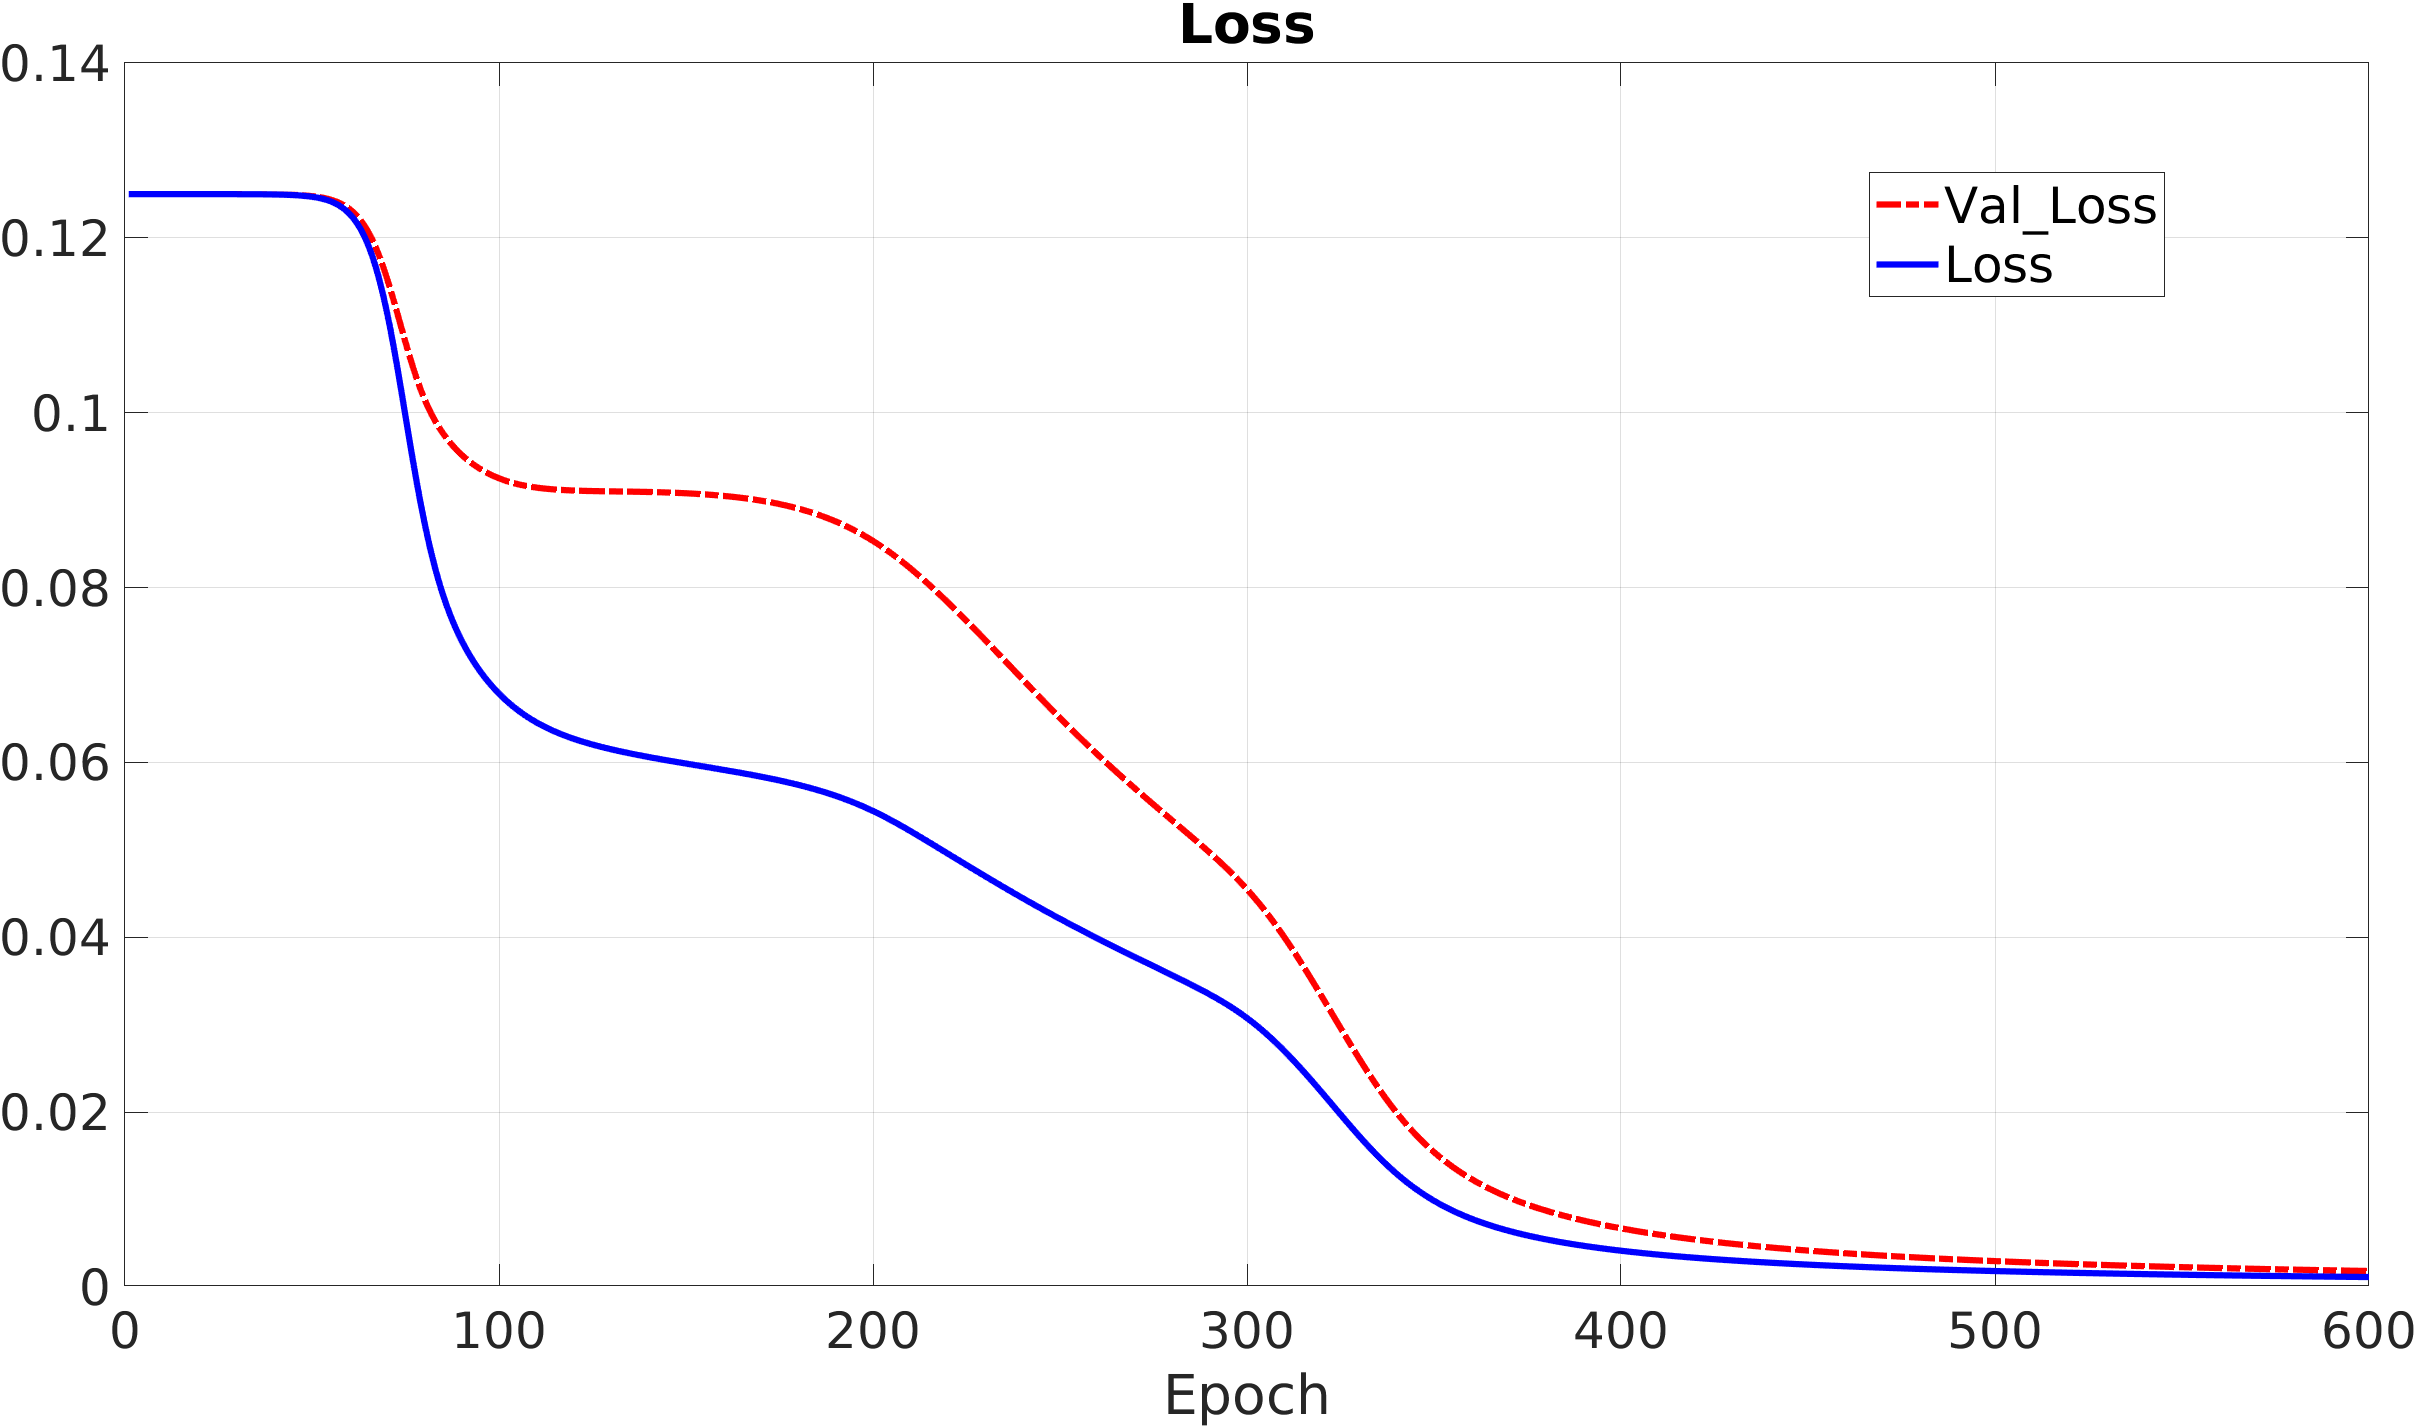
\includegraphics[width=\linewidth]{img/Monk1_loss.png}
        %\subcaption{MSE}
    \end{minipage}%
    \begin{minipage}[t]{0.5\linewidth}
        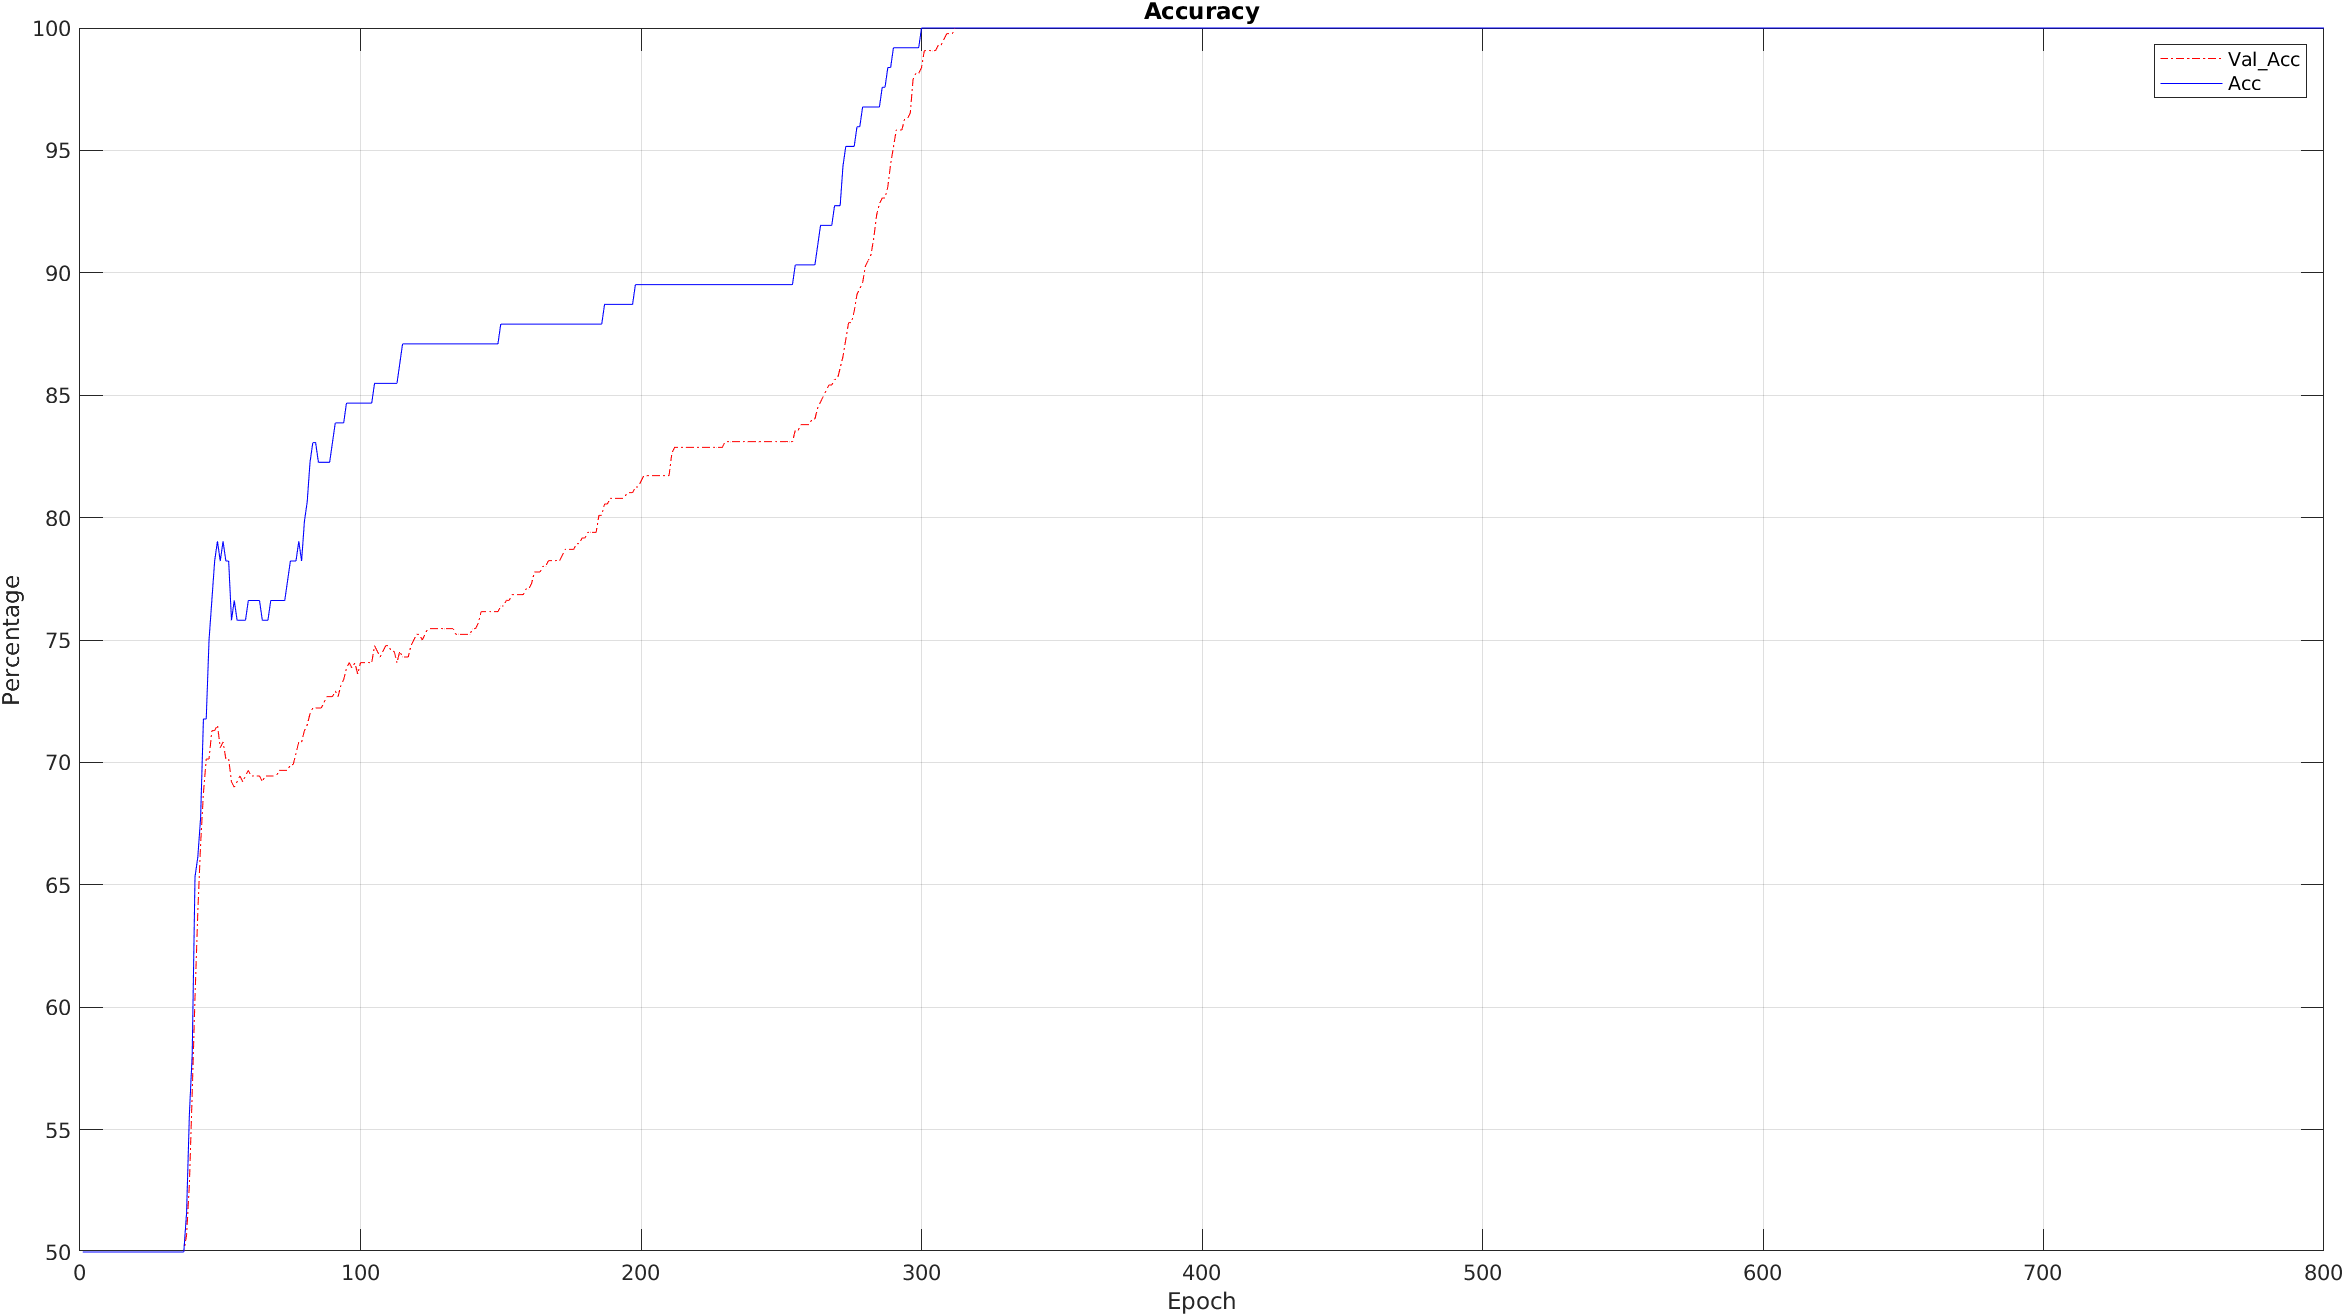
\includegraphics[width=\linewidth]{img/Monk1_accuracy.png}
        %\subcaption{Accuracy}
    \end{minipage}
    \caption{MSE and accuracy for MONK’s 1.}
\end{figure}

\subsubsection{MONK 2}
\begin{figure}[H]
    \centering
    \begin{minipage}[t]{0.5\linewidth}
        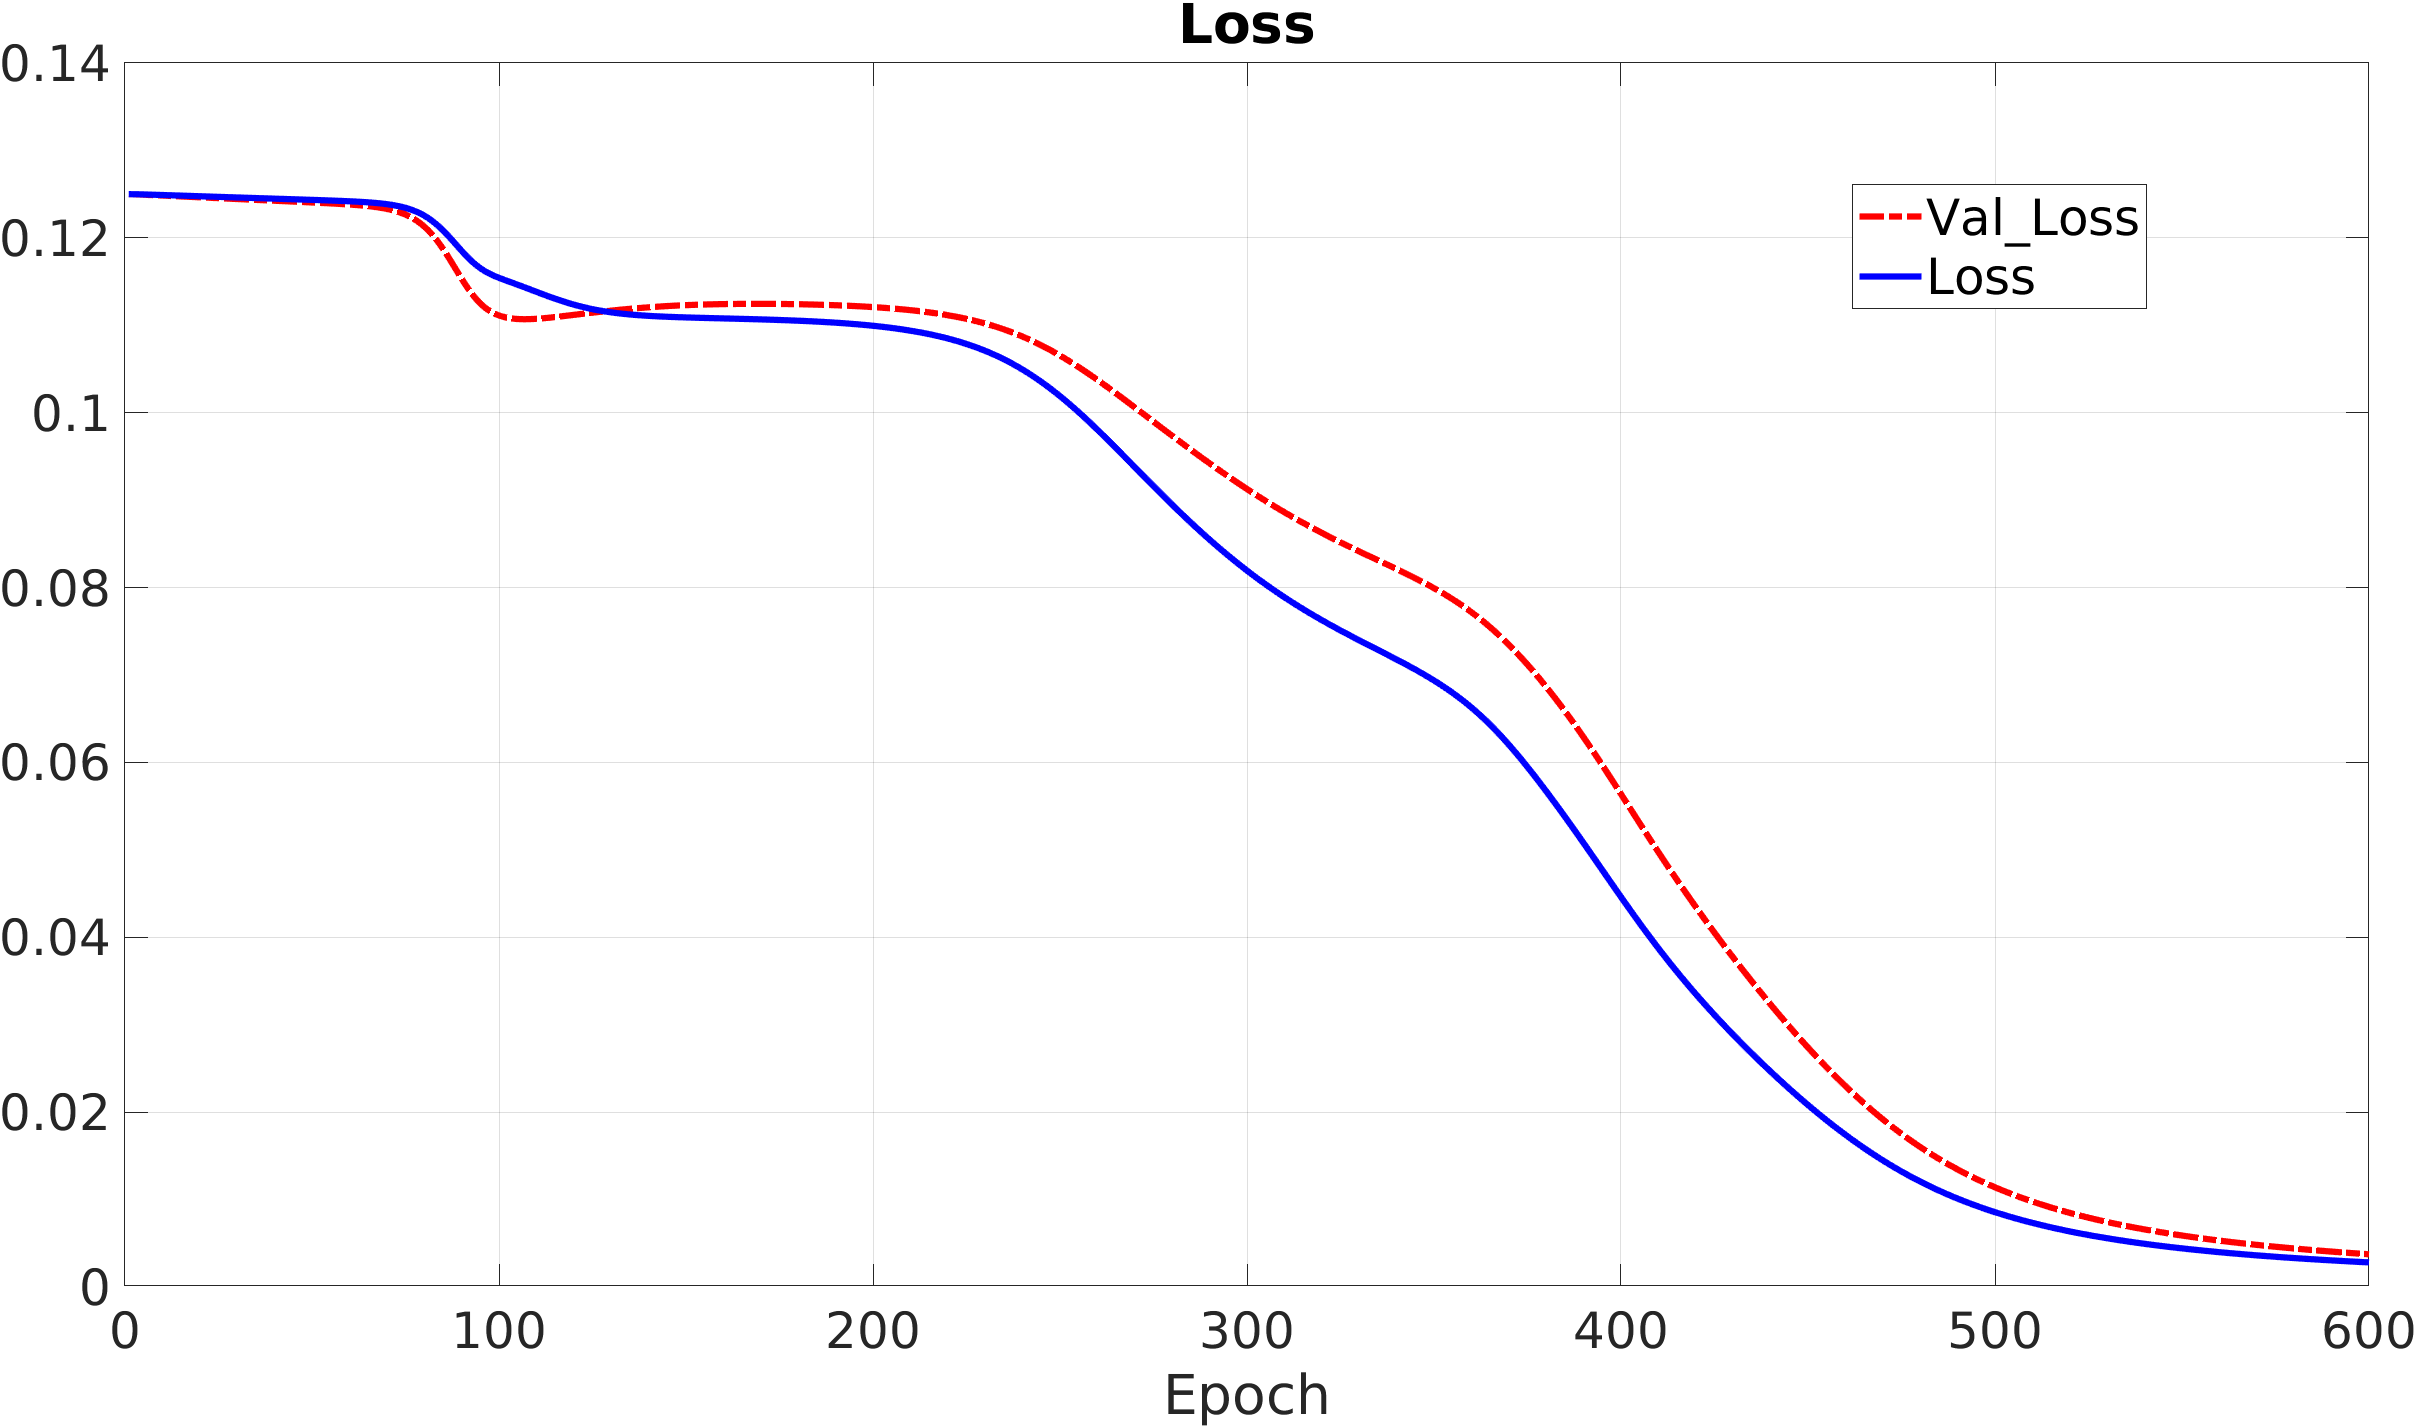
\includegraphics[width=\linewidth]{img/Monk2_loss.png}
        %\subcaption{MSE}
    \end{minipage}%
    \begin{minipage}[t]{0.5\linewidth}
        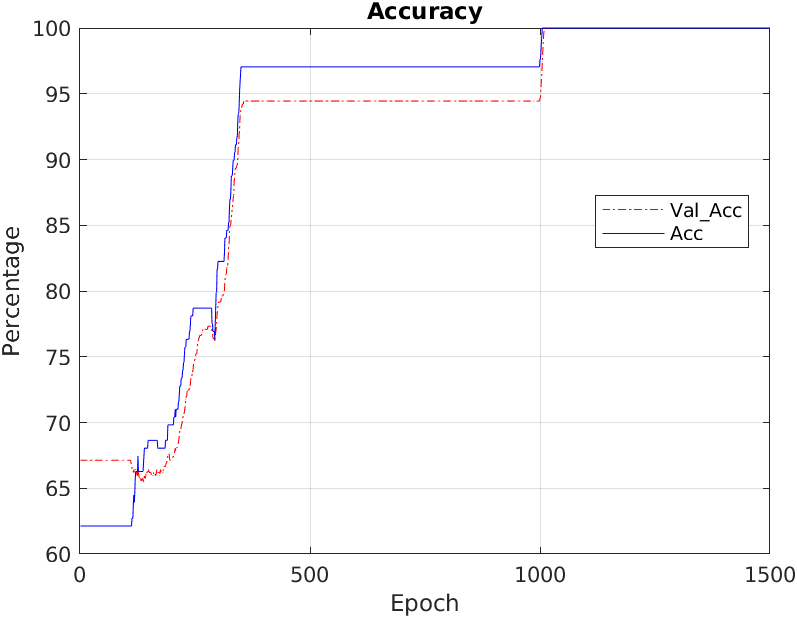
\includegraphics[width=\linewidth]{img/Monk2_accuracy.png}
        %\subcaption{Accuracy}
    \end{minipage}
    \caption{MSE and accuracy for MONK’s 2.}
\end{figure}

\subsubsection{MONK 3}
We figured out during training phase that learning curves of MONK's 3 without regularization shown overfits in the output (see fig. \ref{fig:m3nr}). After that we tried with regularization and we obtained better results, the training didn't show overfitting in the validation error.
\begin{figure}[H]
    \centering
    \begin{minipage}[t]{0.5\linewidth}
        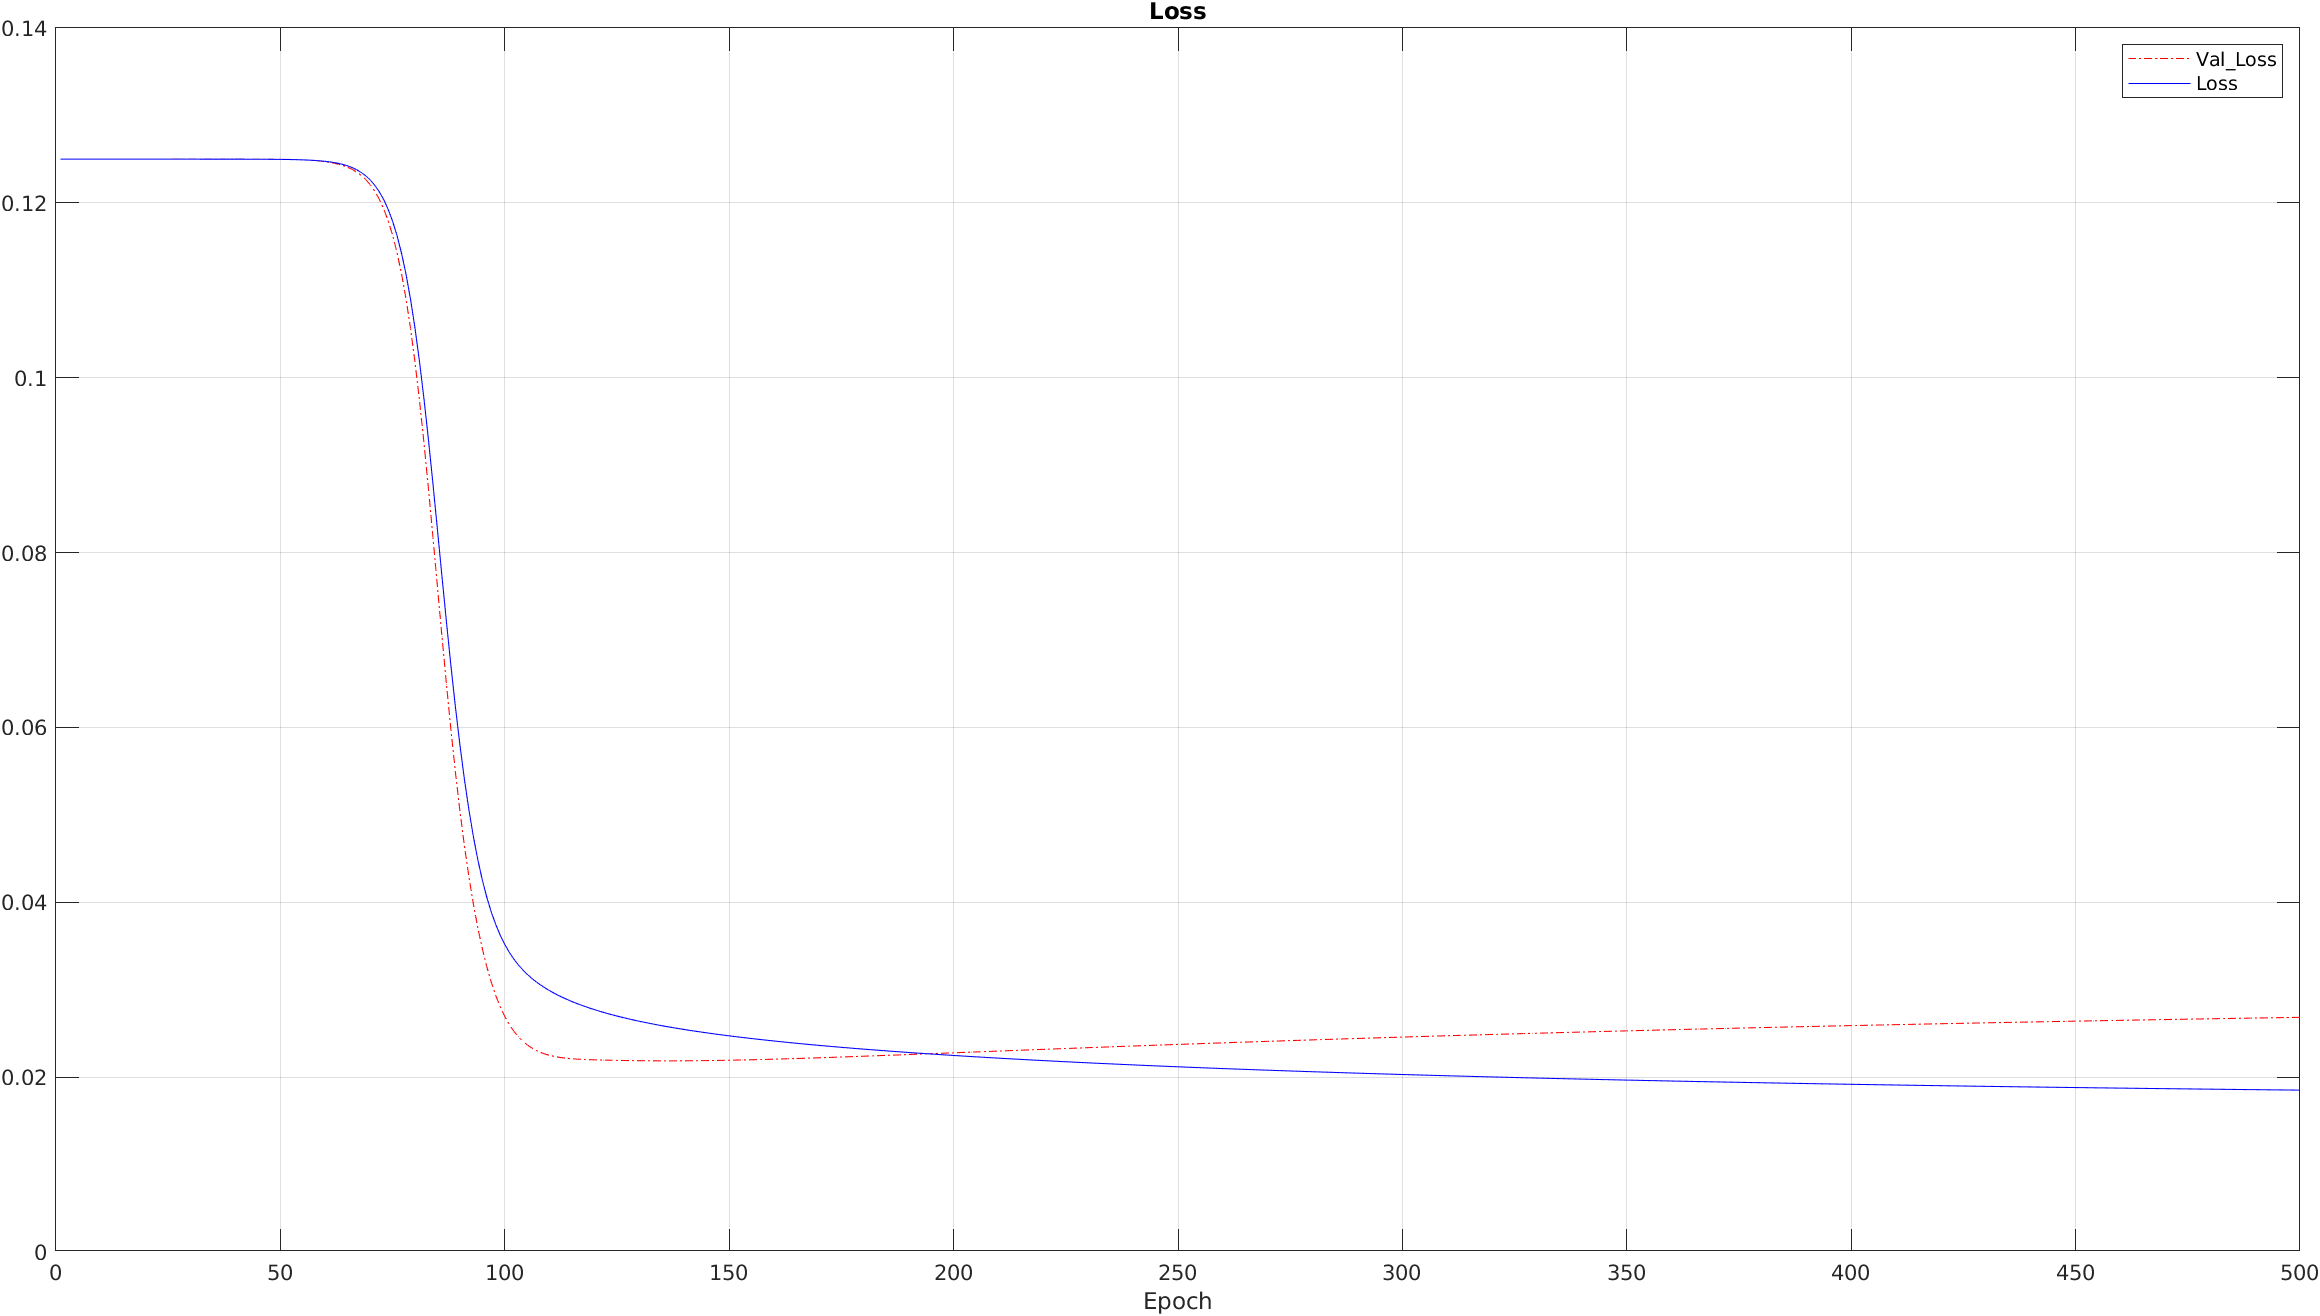
\includegraphics[width=\linewidth]{img/Monk3_loss_noReg.png}
        %\subcaption{MSE}

    \end{minipage}%
    \begin{minipage}[t]{0.5\linewidth}
        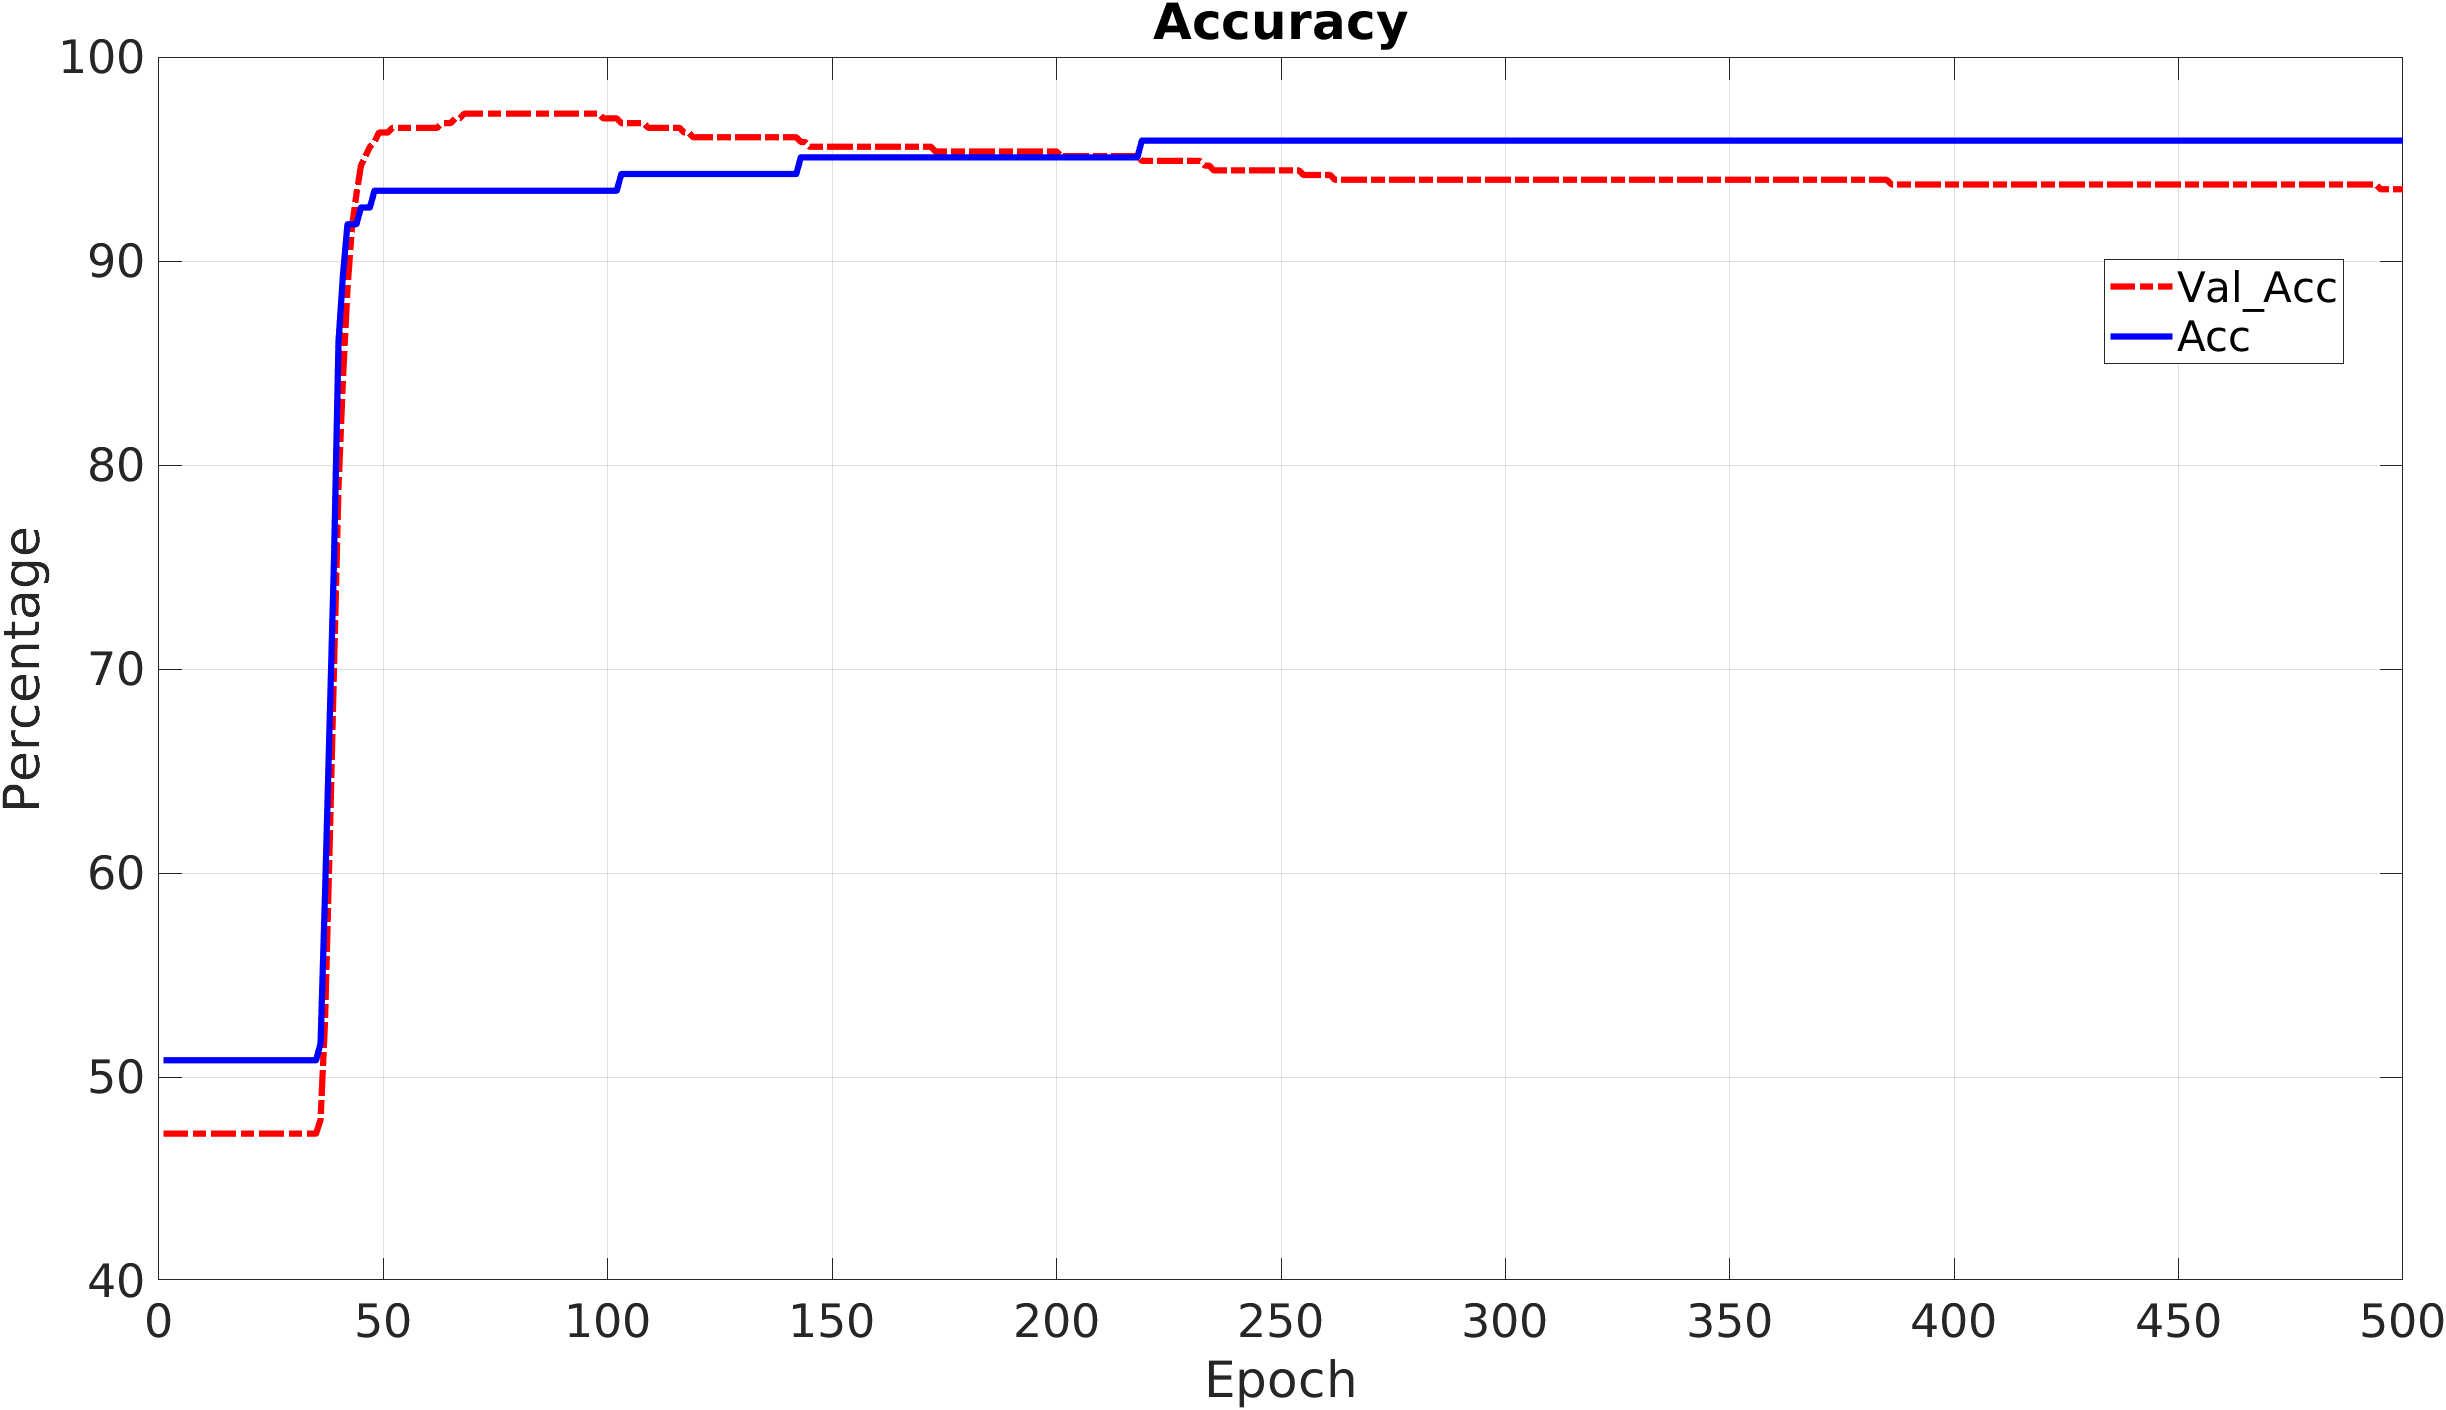
\includegraphics[width=\linewidth]{img/Monk3_accuracy_noReg.png}
        %\subcaption{Accuracy}
    \end{minipage}
    \caption{MSE and accuracy for MONK’s 3 not regularized.}
    \label{fig:m3nr}
\end{figure}

\begin{figure}[H]
    \centering
    \begin{minipage}[t]{0.5\linewidth}
        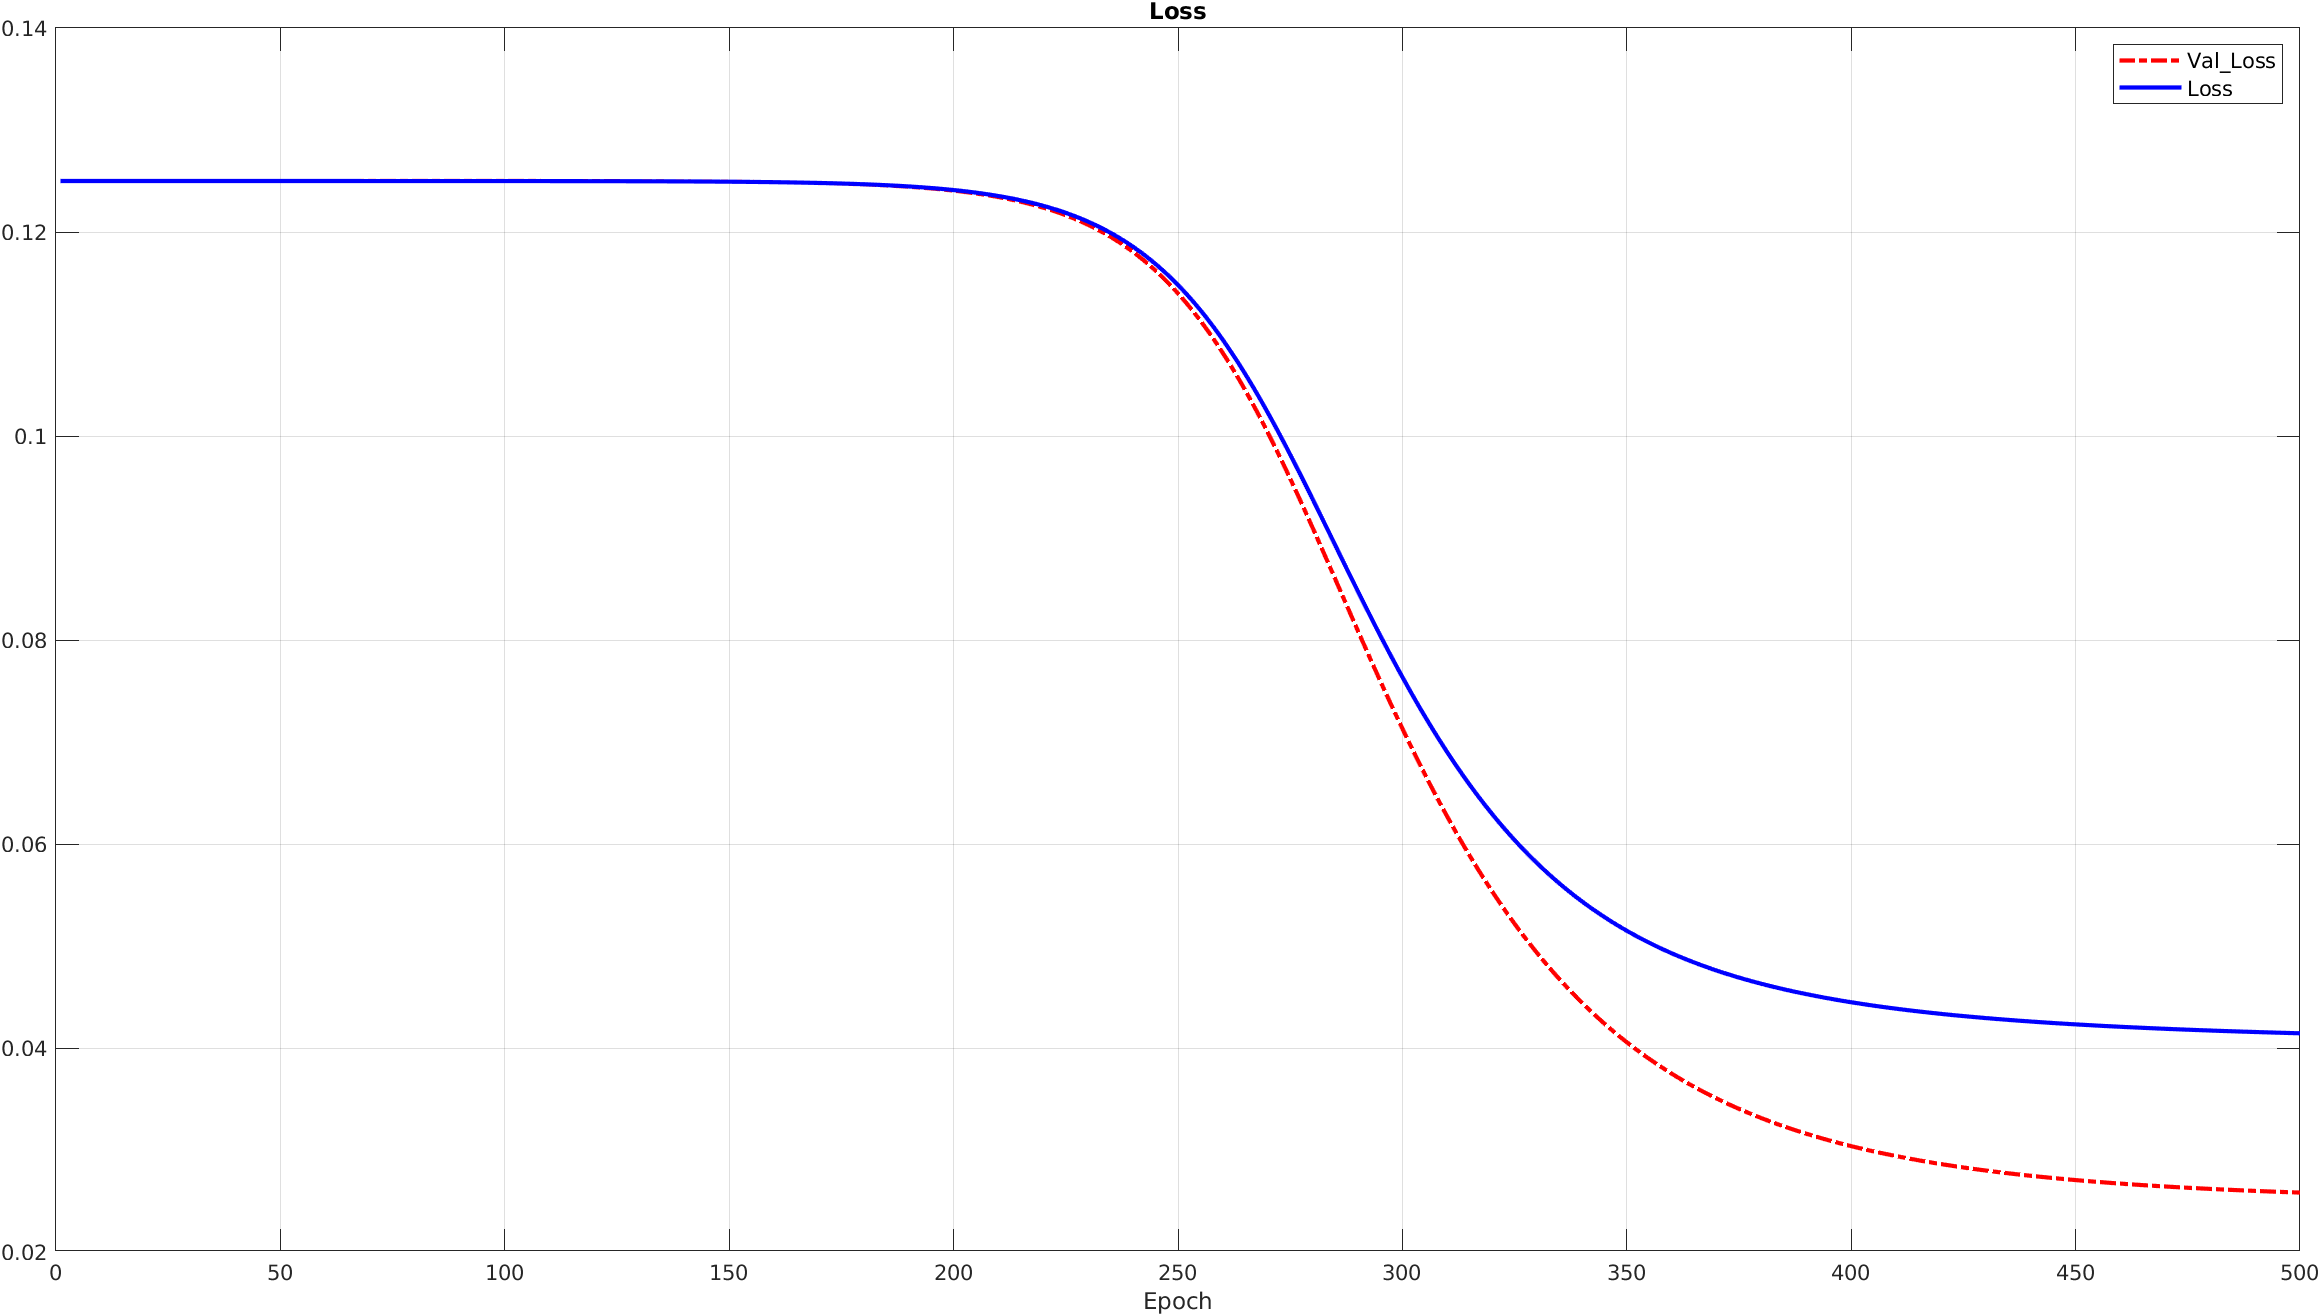
\includegraphics[width=\linewidth]{img/Monk3_loss_Reg.png}
        %\subcaption{MSE}
    \end{minipage}%
    \begin{minipage}[t]{0.5\linewidth}
        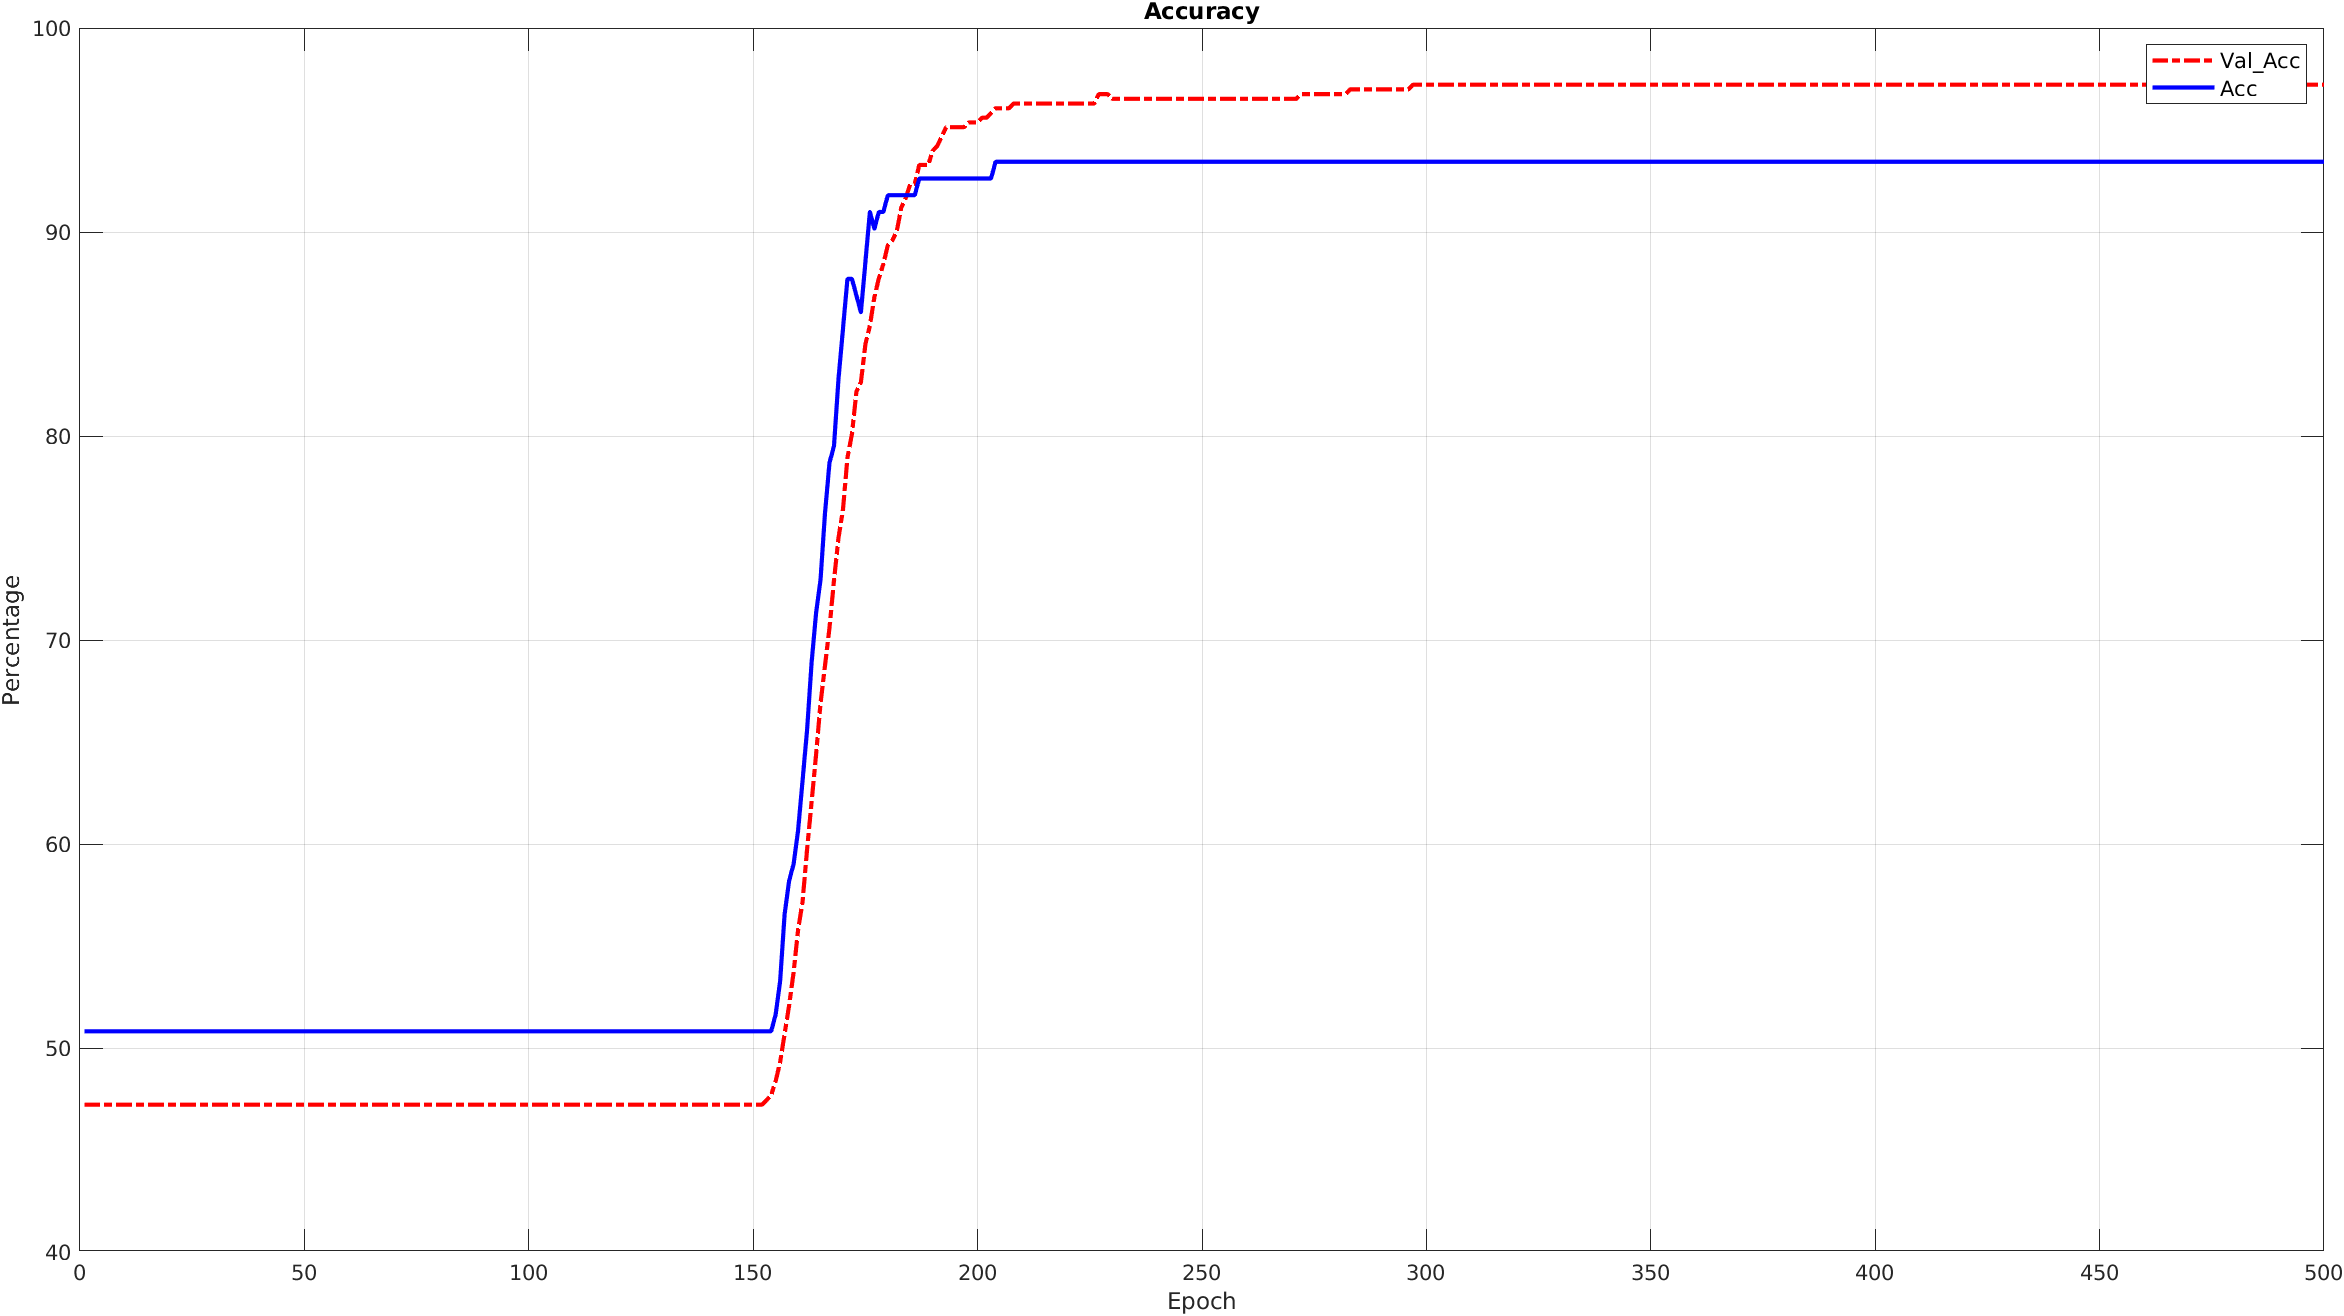
\includegraphics[width=\linewidth]{img/Monk3_accuracy_Reg.png}
        %\subcaption{Accuracy}
    \end{minipage}
    \caption{MSE and accuracy for MONK’s 3 regularized.}
\end{figure}



\subsection{Cup results}

\subsubsection{Validation schema}

At the beginning, we splitted the dataset in training set and test set with 80\% for training and 20\% for test. For the selection of the best model, we decided to use k-fold cross validation with k equals three. In the end we chose the best models among all the models trained during the grid search step. We used stochastic, mini-batch and batch gradient descent and we figured out that the batch type had smoother learning curves.

\subsubsection{Screening phase}

Firstly we tried networks with single hidden layer and we noticed that they had good results. For this reason we tuned the hyper-parameters for this type of network through grids search.
Then we chose MEE as the loss function for validation and test set, we trained the network with MSE but we plot the results with MEE to be comparable with the learning curves of test and validation set.
Next, we focused on find some variant of the network with more hidden layer, we did hyper-parameters tuning through grids search.

\subsubsection{Explored hyper-parameters}
At the beginning, we have done grids search with large interval and high step among them. When we found the right interval we started grids search for each combination of the values:

\begin{itemize}
	\item Unit $\in$ \{25, 200\} with step $\in$ \{25, 50\};
	\item Learning rate $\in$ \{0.0001, 0.01\} with step $\in$ \{0.0001, 0.001\};
	\item Lambda $\in$ \{0, 0.004\} with step $\in$ \{0.0001,  0.0005\};
	\item Momentum $\in$ \{0, 0.8\} with step $\in$ \{0.05,  0.1\}.
\end{itemize}
\vspace{0.3cm}
We used \texttt{tanh} activation function for all hidden layer and \texttt{linear} activation function in the output layer. \texttt{Tanh} was chosen because it had the best result among other results we obtained in previous grid search. \texttt{Linear} was chosen because is often used as output layer activation function for regression problem.

\subsubsection{Grid search result}
The table \ref{tab:best_nets} reports the average of the value found for TR, VS and TS during the k-fold cross validation with k equals three.   
\begin{center}
\small\addtolength{\tabcolsep}{-3pt}
\begin{table}[h!]
	\centering
	\begin{tabular}{|c|c|c|c|c|c|c|c|}
		\hline
		\textbf{Layer}& \textbf{Units}& \textbf{Learning rate} & \multicolumn{1}{l|}{\textbf{Lambda}} & \textbf{Momentum} & \textbf{Error TR}& \textbf{Error VS}& \textbf{Error TS}\\ \hline
			1 & 75 & 0.00450 & 0.00001 & 0.6  & 0.9676 & 1.1202 & 1.2151  \\
			1 & 100 & 0.00087 & 0.0000 & 0.8  & 0.9832 & 1.2750 &  1.2662\\
			1 & 100 & 0.00097 & 0.0000 & 0.8  & 0.9851 & 1.2759 &  1.2786\\
			1 & 100 & 0.00500 & 0.0000 & 0.5  & 0.9859 & 1.2845 & 1.2784 \\
			1 & 100 & 0.00500 & 0.0000 & 0.7  & 0.9752 & 1.2654 & 1.2569 \\
			1 & 100 & 0.00500 & 0.00001 & 0.6  & 0.8731& 1.2412 & 1.2375 \\
			2 & 150 & 0.00875 & 0.0002 & 0.8  & 0.8467 & 1.1332 &  1.1372 \\
			5 & 375 & 0.00450 & 0.0001 & 0.7  & 0.6323 & 1.1341 &  1.1341 \\
		  \hline
	\end{tabular}
		\caption{Best networks configuration with MEE.}
		\label{tab:best_nets}
\end{table}
\end{center}
The two models with more than one hidden layers have the following structure:
\begin{itemize}
	\item Two hidden layer: 100-50-2 (see fig. \ref{img::twolayer});
	\item Five hidden layer: 100-100-75-50-50-2 (see fig. \ref{img::fivelayer}).
\end{itemize}
RIFARE GRAFICI!!!!!!!!!!!!!!!!!!
\vspace{0.5cm}
\begin{figure}[H]
	\centering
	\begin{minipage}[t]{0.5\linewidth}
		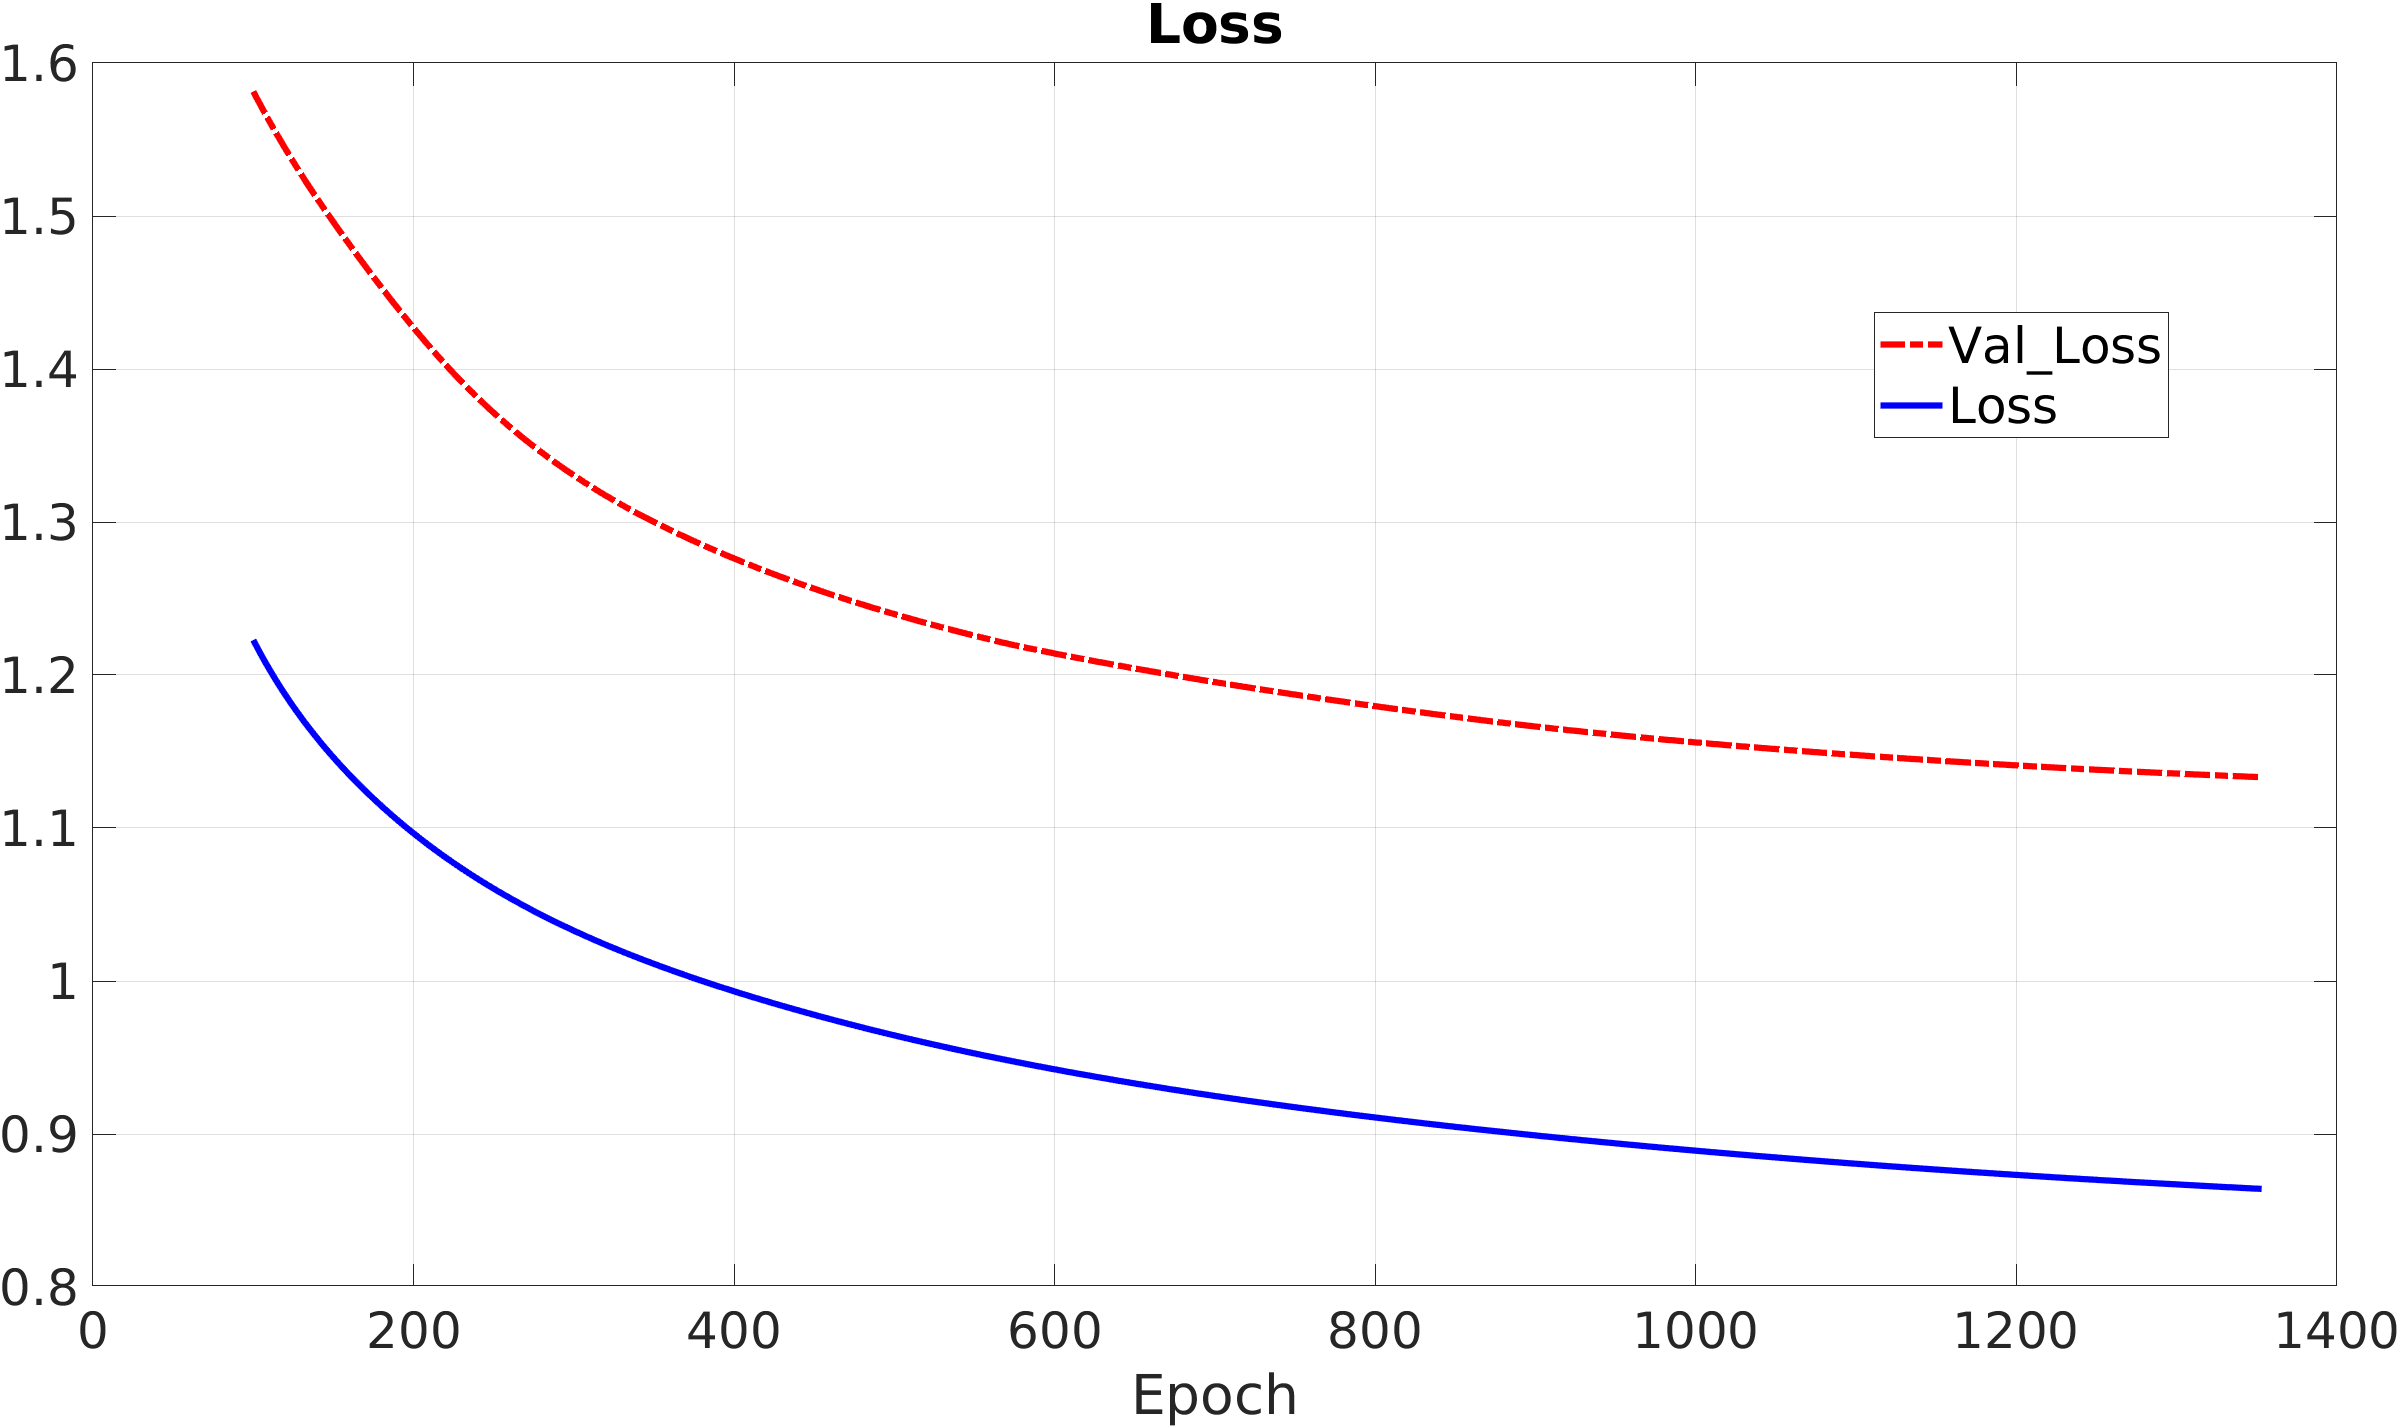
\includegraphics[width=\linewidth]{img/Cup_loss_Reg_Zoom_2l.png}
		\caption{MEE two hidden layer model}
		\label{img::twolayer}
	\end{minipage}%
	\begin{minipage}[t]{0.5\linewidth}
		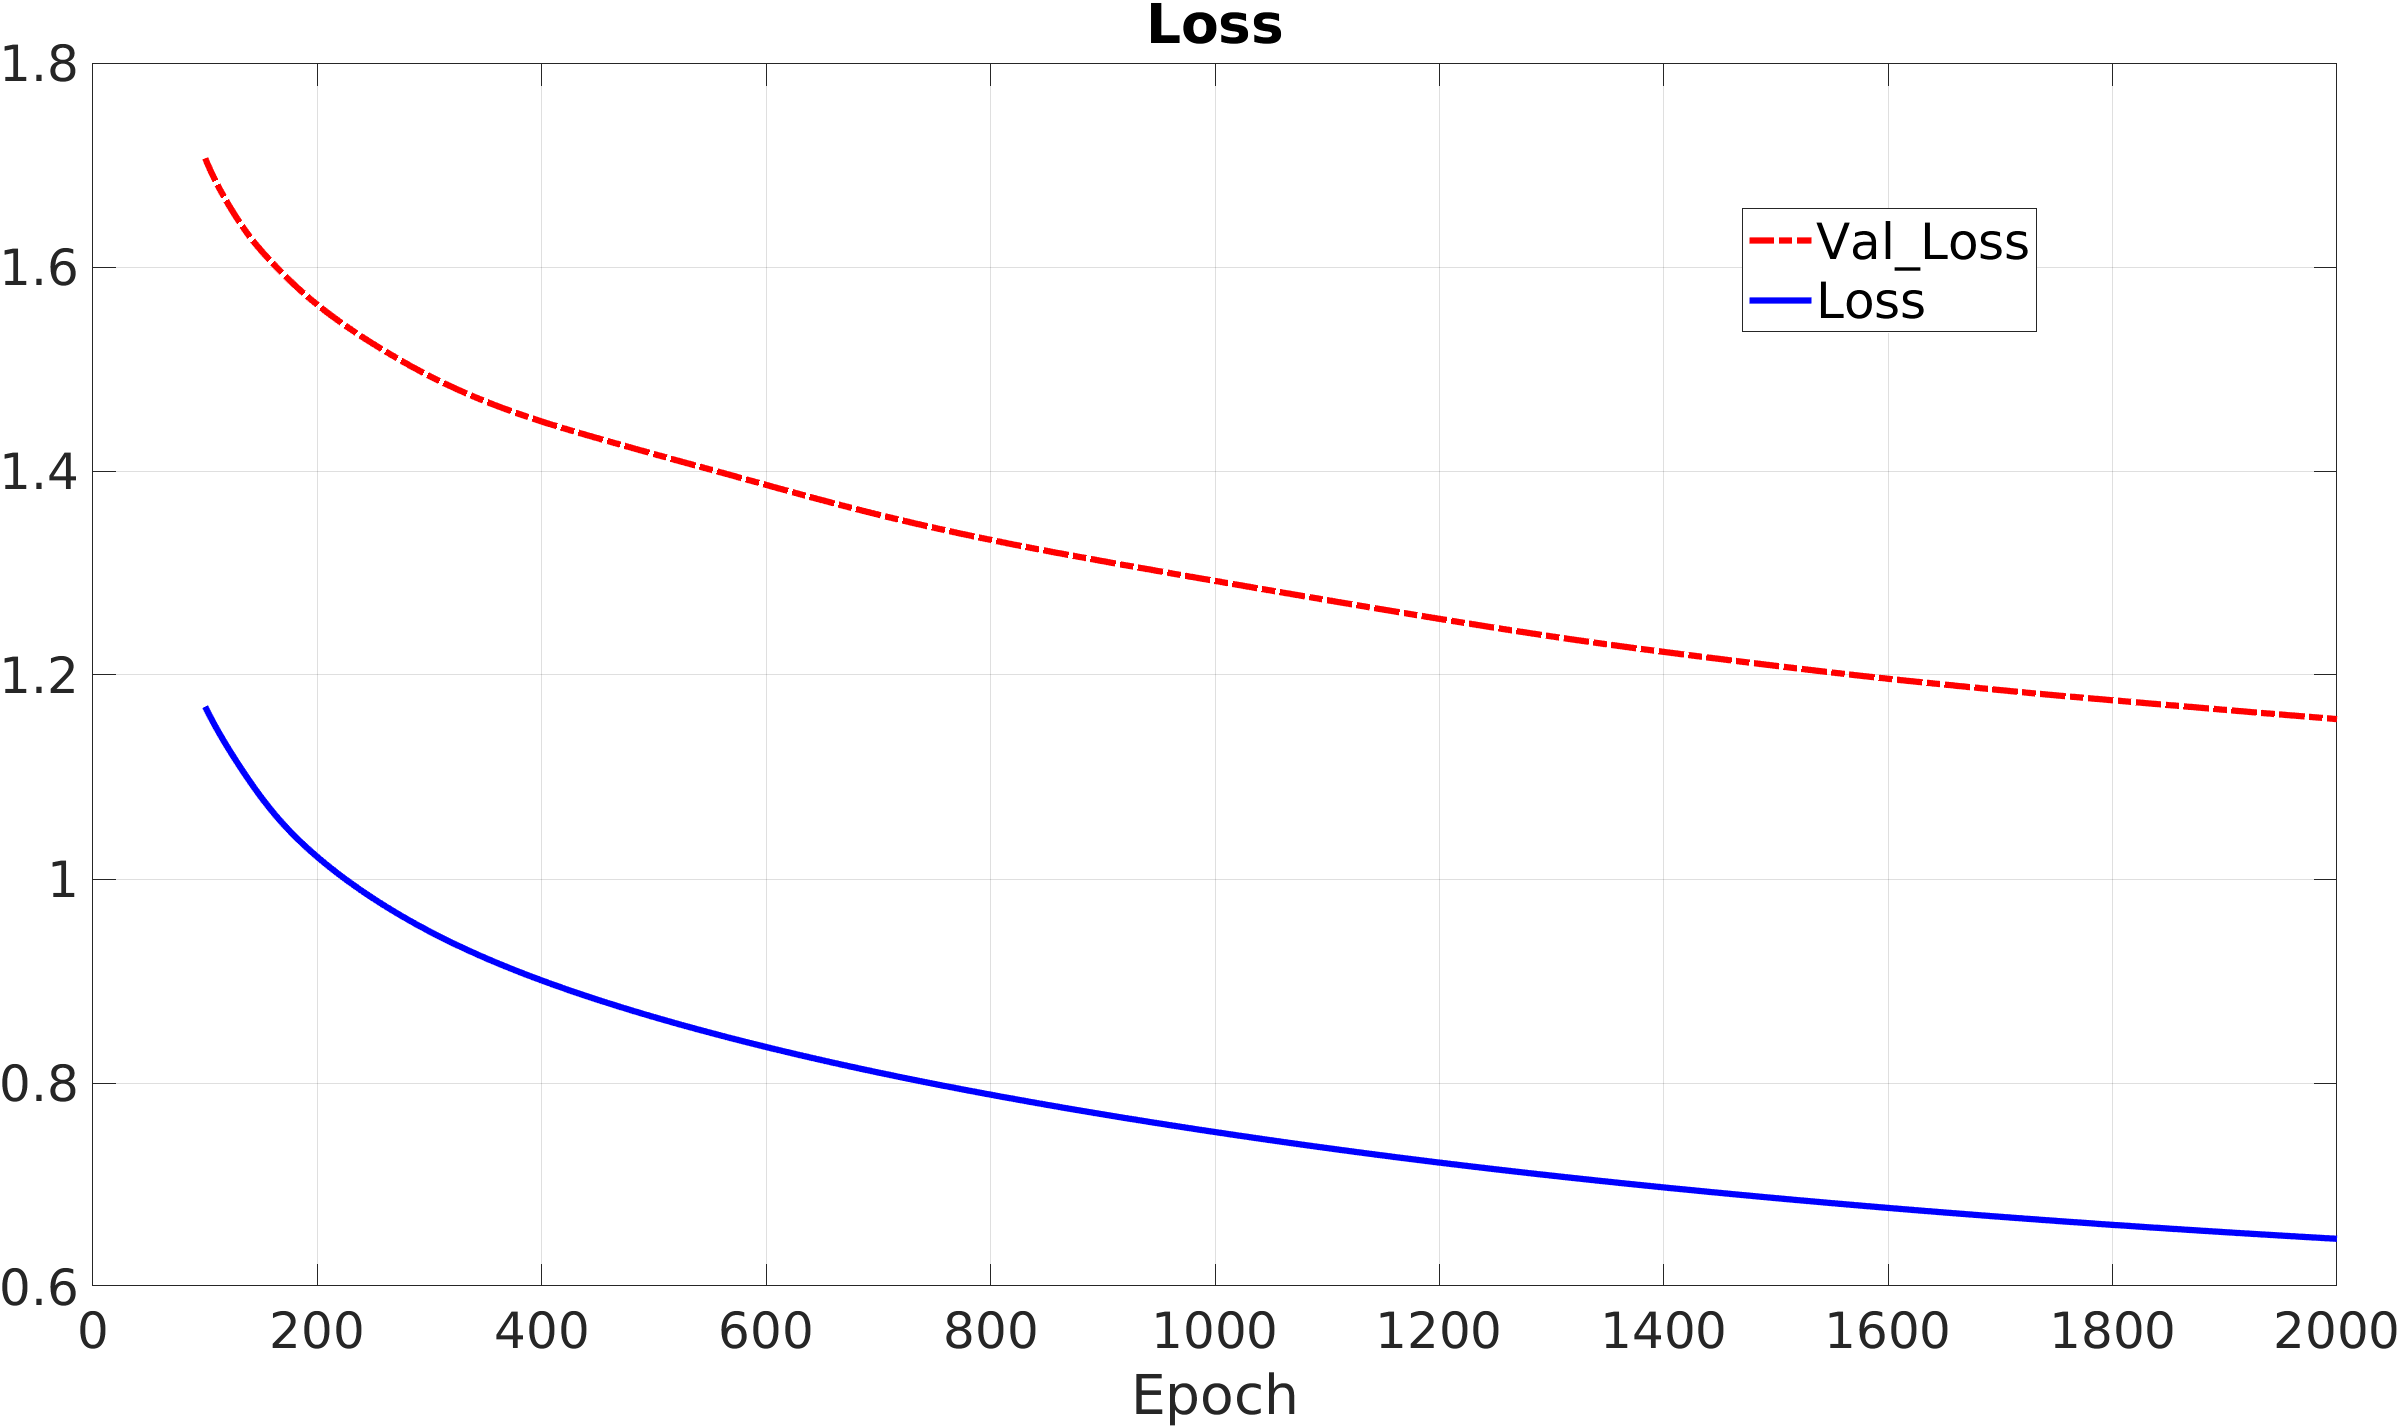
\includegraphics[width=\linewidth]{img/Cup_loss_Reg_Zoom_5l.png}
		\caption{MEE five hidden layer model}
		\label{img::fivelayer}
	\end{minipage}
\end{figure}

\subsubsection{Computing time}
We have developed a parallel grid search that allow us to take advantage of all core of our CPUs automatically. All the computation where launched on the following machine:
\begin{itemize}
	\item Intel i7-8500Y, 1.5GHz;
	\item Intel i7-4720HQ, 2.6GHz.
	
\end{itemize}

The project was developed in C++ and the computational time and memory had to be strictly controlled.
The time it takes to train on the MONK dataset with 800 epoch is 1.5 second, for the ML CUP dataset with 8000 epoch and 75 units is 1.10 minutes.

\subsubsection{Comparisons}
We have tried different neural networks with different number of layer and distinct type of gradient descent (stochastic, mini-batch and batch). We figured out that the number of layers does not significantly affect network generalization performance, moreover with batch gradient descent we got the best learning curve.

\subsubsection{Chosen model}
The final model was chosen from the best models found after the grid search (table \ref{tab:best_nets}), it has the following hyperparameters (table \ref{tab:best_net}) and MEE error for training set, validation set and test set.
We achieved an average MEE of 1.2093 on our test set, taken as an average of seven
different trainings of the networks (to avoid the bias due to the random weight
initialization).
\begin{center} 
\small\addtolength{\tabcolsep}{-3pt}
\begin{table}[h!]
	\centering
	\begin{tabular}{|c|c|c|c|c|c|c|c|}
		\hline
		\textbf{Layer}& \textbf{Units}& \textbf{Learning rate} & \multicolumn{1}{l|}{\textbf{Lambda}} & \textbf{Momentum} & \textbf{Error TR}& \textbf{Error VS}& \textbf{Error TS}\\ \hline
		1 & 75 & 0.00450 & 0.00001 & 0.6  & 0.9676 & 1.1202 & 1.2093  \\
		\hline
	\end{tabular}
	\caption{Best network configuration with MEE.}
	\label{tab:best_net}
\end{table}
\end{center}

We chose it because it was the model that performed better in the validation set. Also its learning curve was smooth and stable.
The learning curve, also with an enlargement, is shown in the figure \ref{img:best}.


\begin{figure}[H]
    \centering
    \begin{minipage}[t]{0.5\linewidth}
        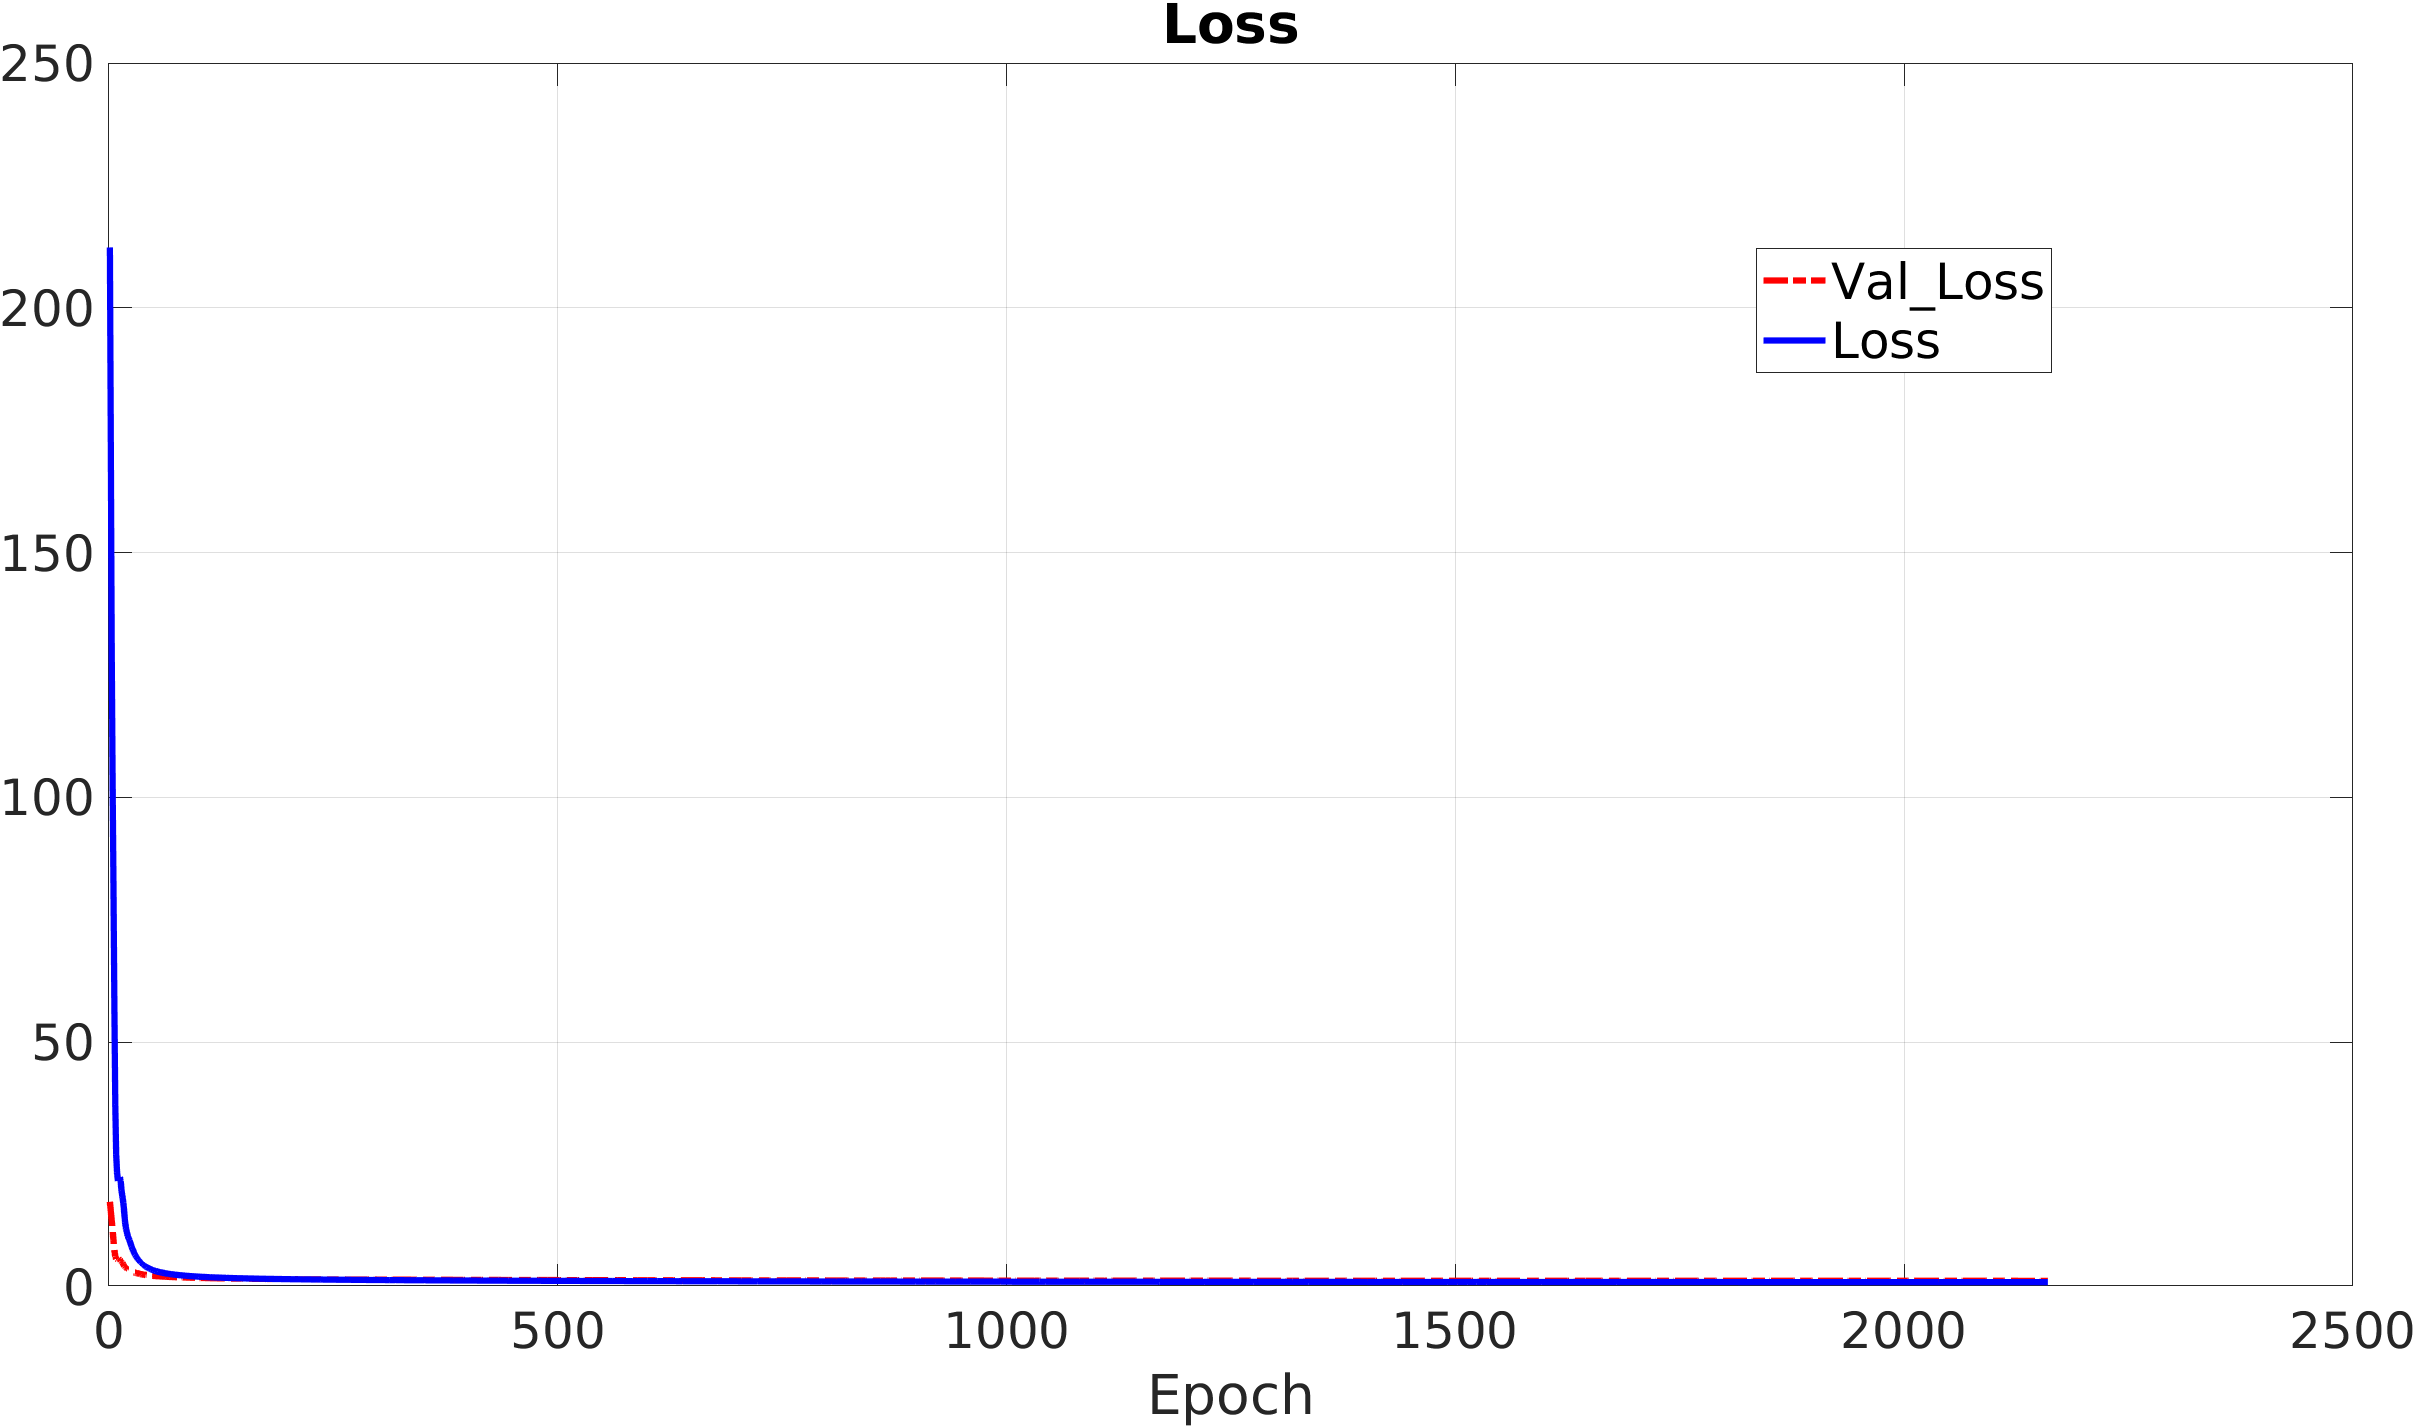
\includegraphics[width=\linewidth]{img/Cup_loss_Reg_noZoom.png}
        %\subcaption{MSE}
    \end{minipage}%
    \begin{minipage}[t]{0.5\linewidth}
        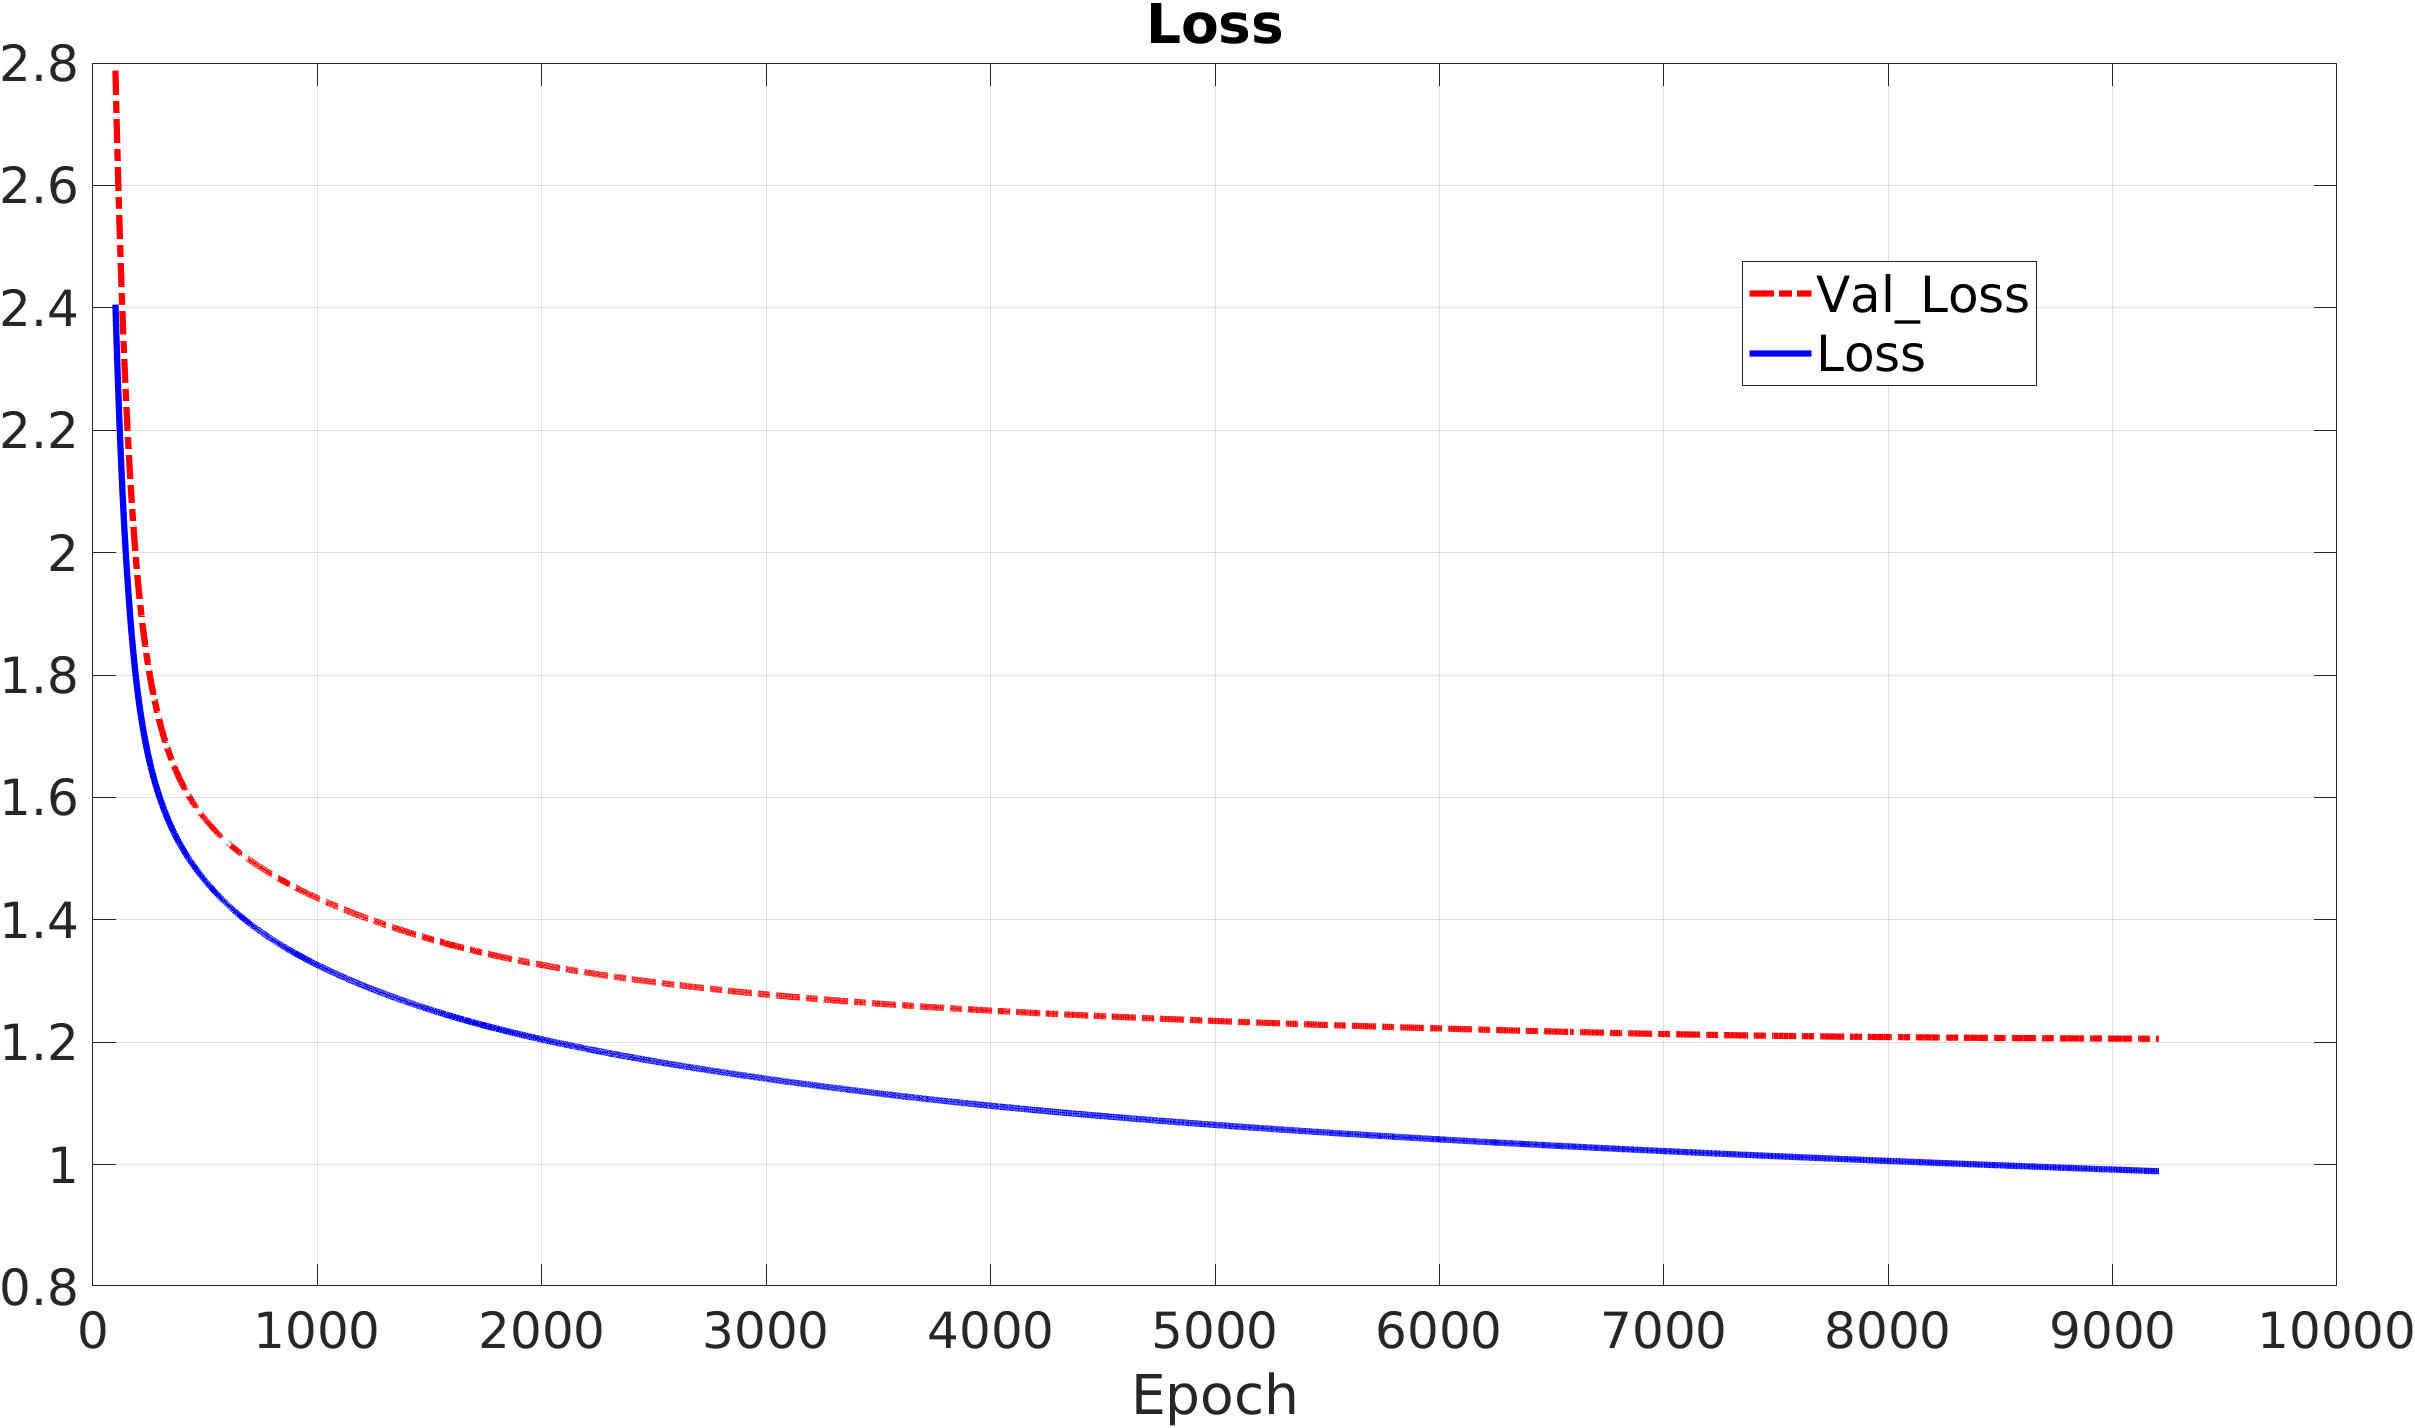
\includegraphics[width=\linewidth]{img/Cup_loss_Reg_Zoom.png}
        %\subcaption{Accuracy}
    \end{minipage}
    \caption{MEE and zoomed MEE for ML cup regularized.}
    \label{img:best}
\end{figure}



